%!TEX program = xelatex
\documentclass[10pt, compress, english]{beamer}

\usetheme[titleprogressbar]{m}

%lyx themes
\usepackage{amsmath}
\usepackage{amssymb}
\usepackage{fontspec}
\setcounter{secnumdepth}{3} 
\setcounter{tocdepth}{3}
\usepackage{float}
\usepackage{graphicx}
\usepackage{esint}
%end lyx themes

 

\usepackage{booktabs}
\usepackage[scale=2]{ccicons}
\usepackage{minted}

\usepgfplotslibrary{dateplot}

\usemintedstyle{trac}

\providecommand{\tabularnewline}{\\}

\makeatletter

%%%% Textclass specific LaTeX commands.
 % this default might be overridden by plain title style
 \newcommand\makebeamertitle{\frame{\maketitle}}%
 % (ERT) argument for the TOC
 \AtBeginDocument{%
   \let\origtableofcontents=\tableofcontents
   \def\tableofcontents{\@ifnextchar[{\origtableofcontents}{\gobbletableofcontents}}
   \def\gobbletableofcontents#1{\origtableofcontents}
 }

\makeatother


\usepackage{xunicode}
\usepackage{polyglossia}

%Margenes personalizadas
\setbeamersize{text margin left=20pt,text margin right=20pt}
 
\begin{document}
%%%%%%%%%%%%%%%%%%%%
%%%%   TITLE   %%%%%
\title[cim@lab]{An Adapted Laplacian Operator For Hybrid Quad/Triangle Meshes}

\subtitle{\textmd{\footnotesize{}A thesis submitted in partial fulfillment
of the requirements for the degree of:}\\
Master in Systems Engineering and Computer Science}

\author[Alexander Pinzón, Eduardo Romero]{Alexander Pinzón Fernández\\
{\footnotesize{}Advisor: Eduardo Romero}}

%\institute[UN]{Universidad Nacional de Colombia\\
%Facultad de Ingeniería\\
%Departamento de Ingeniería de Sistemas e Industrial\\
%Computer Imaging \& Medical Applications Laboratory CIM@LAB}

\date{Bogotá-Colombia. October 2015}

\titlegraphic{
\includegraphics[scale=0.1]{img/logo_cimalab}}
\makebeamertitle

%%%%   END TITLE  %%
%%%%%%%%%%%%%%%%%%%%

\begin{frame}{Outline}

\tableofcontents{}

\end{frame}

\section{Introduction}
\begin{frame}{Spectral Mesh Processing}


Taubin in 1995 suggested that the\textbf{ Discrete Laplace Operator}
allows  \textit{Spectral Processing} on \textbf{Polygonal Meshes}
in an analogous way to signal processing with the Fourier transform.


\begin{center}
\begin{figure}
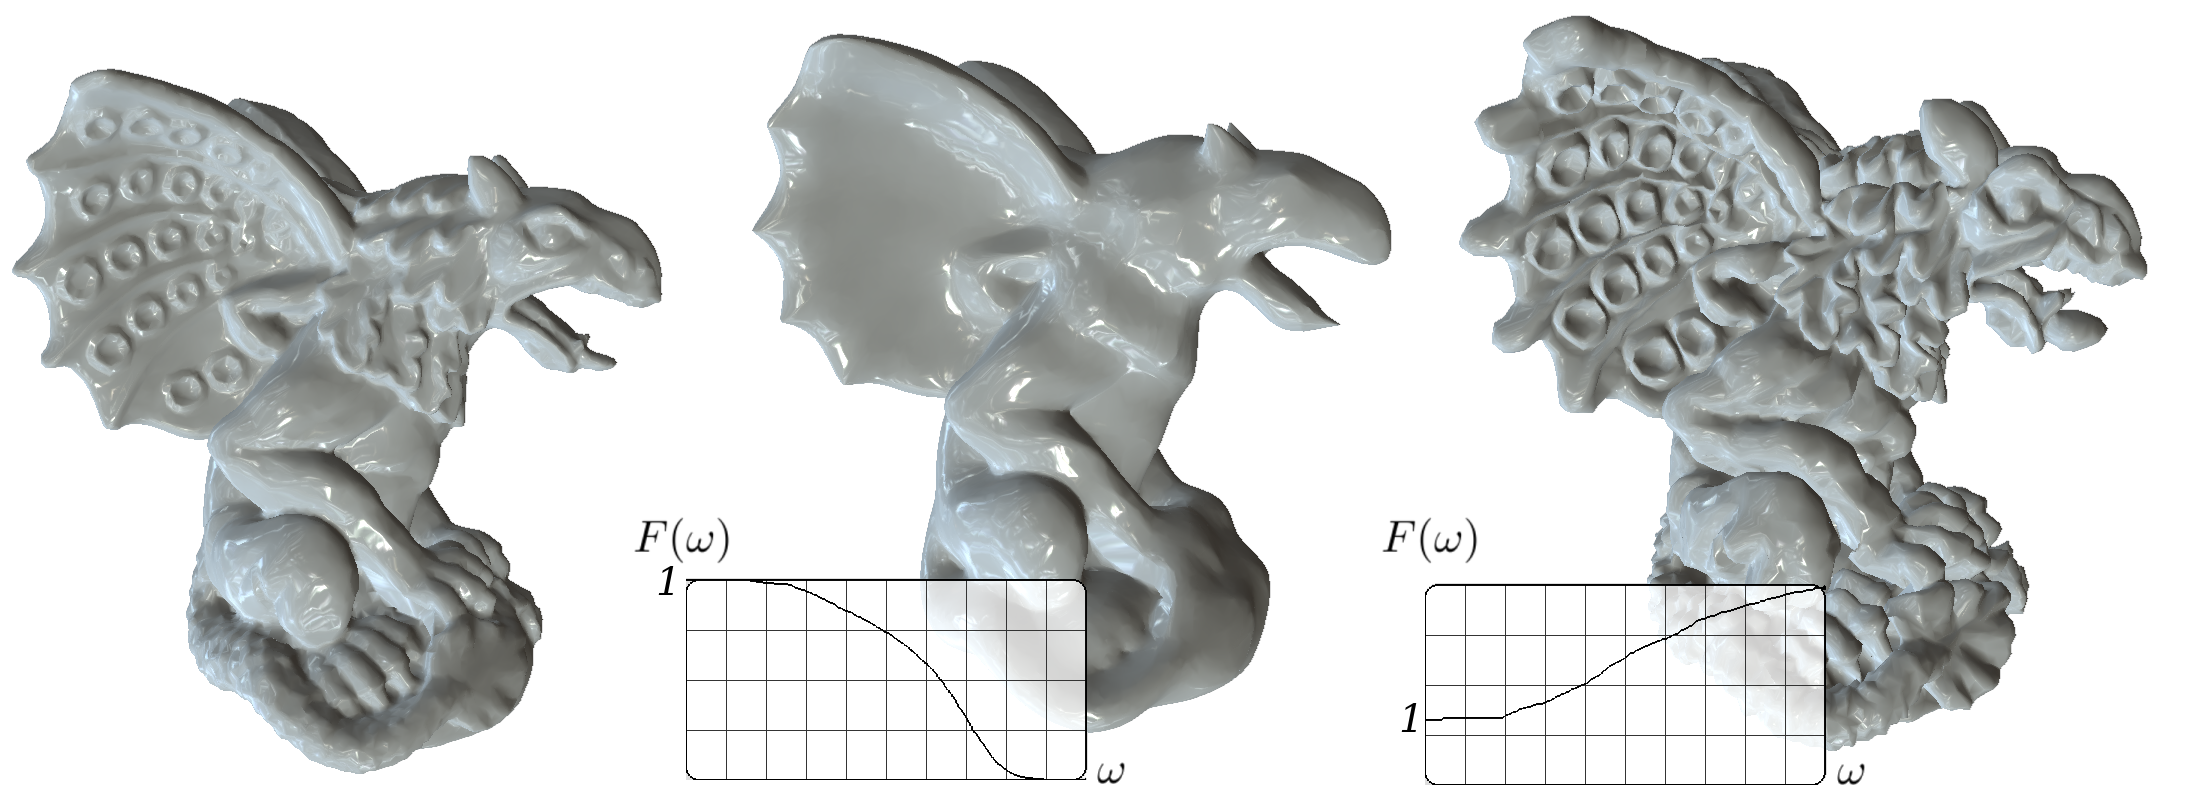
\includegraphics[width=1\textwidth]{img/Gargola_Smoothing_And_Enhance}

\protect\caption{Original Mesh, Low-pass and enhancement filters {[}Vallet08{]}.}
\end{figure}

\par\end{center}


\note[item]{The eigenvalues of Laplace operator are called the \textit{natural
frequencies} and the eigenvectors are called the \textit{natural vibrations}
{[}Taubin 1995{]}.}


\note[item]{WhySpectral? Adifferentwaytolookatfunctionsonadomain}


\note[item]{Taubin in 1995 proposed that is possible to process polygonal meshes
in an analogous way to how signals are processed with the Fourier
transform.\\
En 1995 Taubin propuso que era posible procesar mallas de polígonos
de una manera análoga a como se procesas señales con la transformada
de Fourier. \\
\\
Taubin observo que los componentes en frecuencia de la transformada
de Fourier podían ser descritos como la decomposition of the signal
into a linear combination of the eigenvetors of the Laplacian operador.
\\
\\
Taubin definio un nuevo operador discreto que tomaría el lugar del
operador Laplaciano para suavizar poligonal meshes. \\
\\
Pinkall , Desbrun y otros autores definieron nuevas versiones discretas
del operador Laplaciano pero tomaron en cuenta la definición del Bernoulli
del operador Laplaciano la cual lo toma como la divergencia del gradiente
de una superficie. \\
\\
Hoy dia se cuenta con representaciones discretas del operador de Laplace
Beltrami para procesar mallas de polígonos compuestas por triángulos
o por cuadrángulos Nosotros proponemos una adaptación para poder trabajar
mallas de polígonos hibridas compuestas por triángulos y cuadrángulos
que permitan realizar una aproximación espectral al procesamiento
de mallas de polígonos. }


\note[item]{Taubin (1995) suggested that the frequency components of the Fourier
transform could be described as decomposition of the signal into a
linear combination of the eigenvectors of the Laplacian operator.}

\end{frame}

\begin{frame}{Laplacian of the Fourier transform}


if $\mathbf{u}$ is a eigenfunction and $\lambda$ is a corresponding
eigenvalue of a linear differential operator\textbf{ $\mathbf{A}$}
then


\begin{center}
$\mathbf{Au}=\lambda\mathbf{u},\,\,\,\mathbf{u}\neq0$
\par\end{center}

\pause{}
 
The basis $\mathbf{e}_{w}=\mathbf{e}^{2\pi iwx}=\cos\left(2\pi wx\right)-i\sin\left(2\pi wx\right)$ sine and cosine functions of the Fourier
transform are eigenfunctions of the Laplacian with eigenvalue $\lambda_{w}$ 


\begin{center}
$\Delta\left(\mathbf{e}_{w}\right)=\frac{\partial^{2}}{\partial x^{2}}\mathbf{e}_{w}=-\left(2\pi w\right)^{2}\mathbf{e}_{w}=\lambda_{w}\mathbf{e}_{w}$
\par\end{center}


\begin{center}
$\Delta\left(\mathbf{e}_{w}\right)=\lambda_{w}\mathbf{e}_{w}$
\par\end{center}


\note[item]{Inner product $\left\langle f,\mathbf{e}_{w}\right\rangle $}


\note[item]{A widely used class of linear operators acting on infinite dimensional
spaces are the differential operators on function spaces. Let D be
a linear differential operator on the space \textbackslash{}mathbf\{C\textasciicircum{}\textbackslash{}infty\}
of infinitely differentiable real functions of a real argument t.
The eigenvalue equation for D is the differential equation https://en.wikipedia.org/wiki/Eigenvalues\_and\_eigenvectors\#Generalizations\_to\_infinite-dimensional\_spaces}


\note[item]{Taubin analogy between Fourier transform and eigenvectors of Laplacian
operator}


\end{frame}

\begin{frame}{Laplace-Beltrami operator}



\begin{block}{The Laplace-Beltrami operator $\Delta_{M}$ is a differential operator
given by the divergence of a gradient field on a \textbf{surface}.}


\[
\begin{array}[t]{c}
\frac{\partial^{2}f}{\partial x^{2}}+\frac{\partial^{2}f}{\partial y^{2}}+\frac{\partial^{2}f}{\partial z^{2}}=0\\
\nabla_{M}^{2}f=\Delta_{M}=0\\
\Delta_{M}=div\left(\nabla_{M}f\right)
\end{array}
\]


where $M$ is a compact and smooth \textbf{Surface} (2D-Manifold).
\end{block}

\pause{}

The Laplace-Beltrami is a generalization of the Laplace operator for functions over surfaces and allows spectral surface analysis.


\note[item]{The LBO is a generalization of the Laplace operator to surfaces.\\
and $f$ is twice differentiable function\\
This operator allows modeling the behavior of complex applications
such as noise reduction, enhancement, remeshing, UV mapping, posing,
skeletonization, among others, in a simple way.}

\end{frame}

\begin{frame}{Surface}


\centering

\begin{minipage}[c]{0.48\columnwidth}%
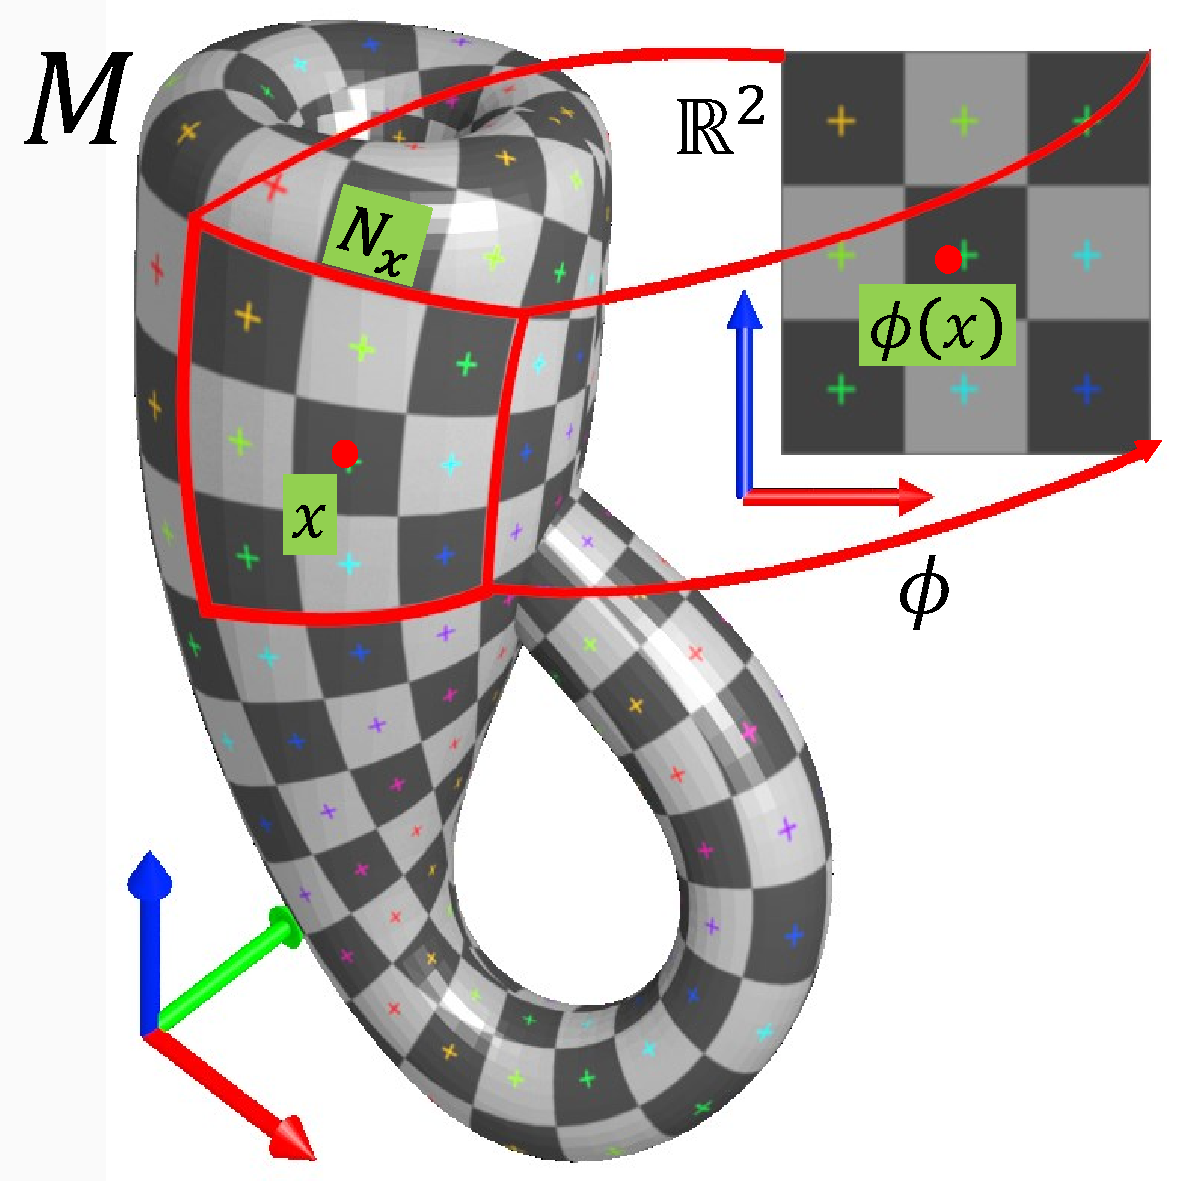
\includegraphics[width=1\columnwidth]{img/Manifolds}%
\end{minipage}\hspace{2bp}%
\begin{minipage}[c]{0.48\columnwidth}%
\vspace{40bp}


A Surface $M$ is a 2D topological manifold.

For which every point $x\in M\subseteq\mathbb{R}^{3}$ has a neighborhood
$N_{x}$ homeomorphic to euclidean space $\mathbb{R}^{2}$.

\begin{center}
A homeomorphism $\phi:\,\,\, N_{x}\rightarrow\mathbb{R}^{2}$
\par\end{center}%
\end{minipage}
\end{frame}

\begin{frame}{Surface discretization with polygonal meshes}


\centering


\begin{minipage}[c]{0.48\columnwidth}%
In computer graphics a \textbf{Surface} is often discretized into
a \textbf{Polygonal Mesh}\\


\textbf{Polygonal Mesh} is a set of points that are connected by \textbf{triangles}
and \textbf{quads}.%
\end{minipage}~%
\begin{minipage}[c]{0.48\columnwidth}%
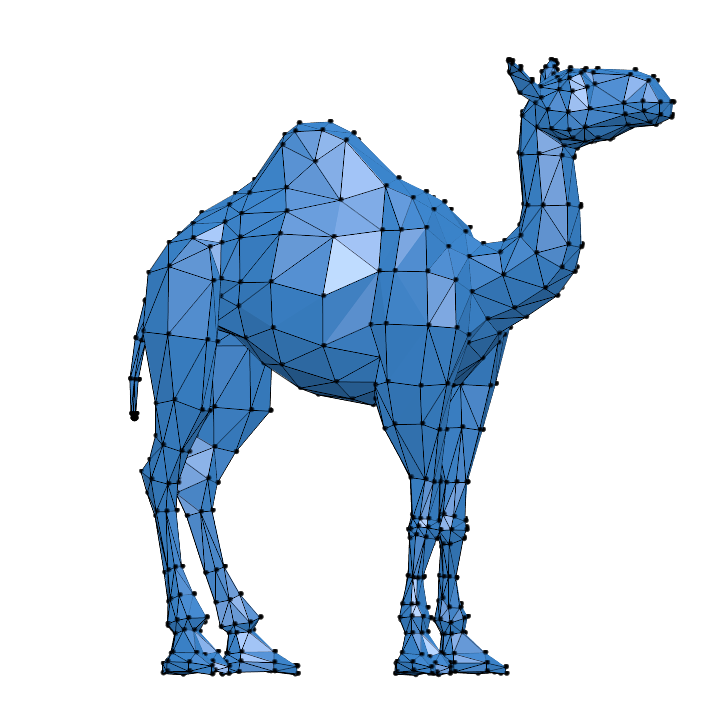
\includegraphics[width=1\columnwidth]{img/Polygon_mesh}%
\end{minipage}

\pause{}

\begin{alertblock}{}
We need discrete versions of Laplacian operator to work with polygonal
meshes.
\end{alertblock}

\note[item]{Since meshes are inherently not smooth we cannot employ classical
calculus methods on these surfaces.}


\note[item]{It is therefore necessary to define a \textbf{discrete Laplacian
operator }that acts on functions defined by such meshes.}

\end{frame}

\begin{frame}{Discrete Laplacian operator as a matrix equation}


\framesubtitle{The discrete version of Laplace operator for polygonal meshes.}


Given a polygonal mesh\textbf{ $\mathbf{M}=\left[v_{1},...\,,v_{n}\right]^{T}$}
and $v_{i}\in\mathbb{R}^{3}$ we define the \textbf{Discrete Laplacian
operator matrix} $L$ with size $n\times n$


\begin{center}
$L\left(i,j\right)=\begin{cases}
w_{ij} & \mbox{if }j\in N\left(v_{i}\right)\\
\sum w_{ik} & \mbox{if }i=j\\
0 & \mbox{otherwise}
\end{cases}$
\par\end{center}


$w_{ij}$ are the weights between the vertex $v_{i}$ and vertex $v_{j}$.
The weights are define depending on the polygonal structure and application.


\textcolor{white}{\tiny{}.}{\tiny \par}


$N\left(v_{i}\right)$ is the 1-ring neighborhood with shared face
to vertex $v_{i}$.


\note[item]{Debido a estas propiedades a matrix L puede tener sus eigenvetores
y cumplir esta propiedad.}


\note[item]{similar to an eigenvector of a matrix $\mathbf{A}\mathbf{e_{i}}=\lambda_{i}\mathbf{e}_{i}$
{[}Botsch 2010{]}.}


\note[item]{Taubin's analogy between the Fourier transform and Laplace Operator.}


\note[item]{Properties of Matrix $L$:}


\note[item]{• Symmetry}


\note[item]{• Positive Weights.}


\note[item]{• Positive Semi-Definiteness}


\note[item]{In polygonal meshes, spectral structure is calculated using the eigenvectors
of the discrete versions of the Laplace-Beltrami operator.}


\note[item]{The weights are define depending of the polygonal structure.}


\note[item]{Weights (Herholz2012)Page 21}

\end{frame}

\begin{frame}{Desired properties for Laplacian matrix}


This properties ensure the construction of eigenstructure of Laplacian
matrix and then those eigenvectors of L matrix are an orthogonal basis
of $\mathbb{R}{}^{n}$
\begin{itemize}
\item Symmetry.
\item Square.
\item Locality.
\item Positive Weights.
\item Positive Semi-Definiteness.
\item Convergence.
\end{itemize}
\end{frame}

\begin{frame}{Eigenstructure of Laplacian matrix}


\begin{center}
$L\mathbf{e_{i}}=\lambda_{i}\mathbf{e_{i}},\,\,\,\mathbf{e_{i}}\neq0$
\par\end{center}
\begin{itemize}
\item The eigenvector $\mathbf{e}_{i}$ of $L$ is a \textbf{\textsl{natural
vibration}} of the mesh {[}Taubin95{]}.
\item The frequency of the wave $\mathbf{e}_{i}$ is the eigenvalue $\lambda_{i}$
of $L$ that is the \textbf{\textsl{natural frequency }}{[}Taubin95{]}.
\end{itemize}

\begin{figure}
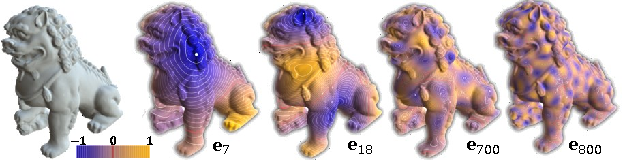
\includegraphics[width=1.0\textwidth]{img/Harmoni_Eigenvectors_dog}

\protect\caption{Color values are the amplitude of a wave $\mathbf{e}_{i}$ projected
on the mesh {[}Vallet08{]}.}


\end{figure}


\note[item]{Since the matrix L is symmetric and positive semi-definite (see Section
A.1), its eigenvectors build an orthogonal basis of IRn, such that
we can exactly represent each vector f = (f1, . . . , fn)T in this
basis: {[}botsh 2010{]}}


\note[item]{la multiplicacion del vector f por un vector base e, lo lleva al
espacio representado por L}


\note[item]{The \textsl{k}th entry of $\mathbf{e}_{i}$ corresponds to the amplitude
of the wave $\mathbf{e}_{i}$ at vertex $v_{k}$.}


\note[item]{Si A: V → V es un operador lineal en un cierto \textbackslash{}scriptstyle
\textbackslash{}mathbb\{K\}espacio vectorial V, v≠0 es un vector diferente
de cero en V y c es un escalar tales que}


\note[item]{• The eigenvectors of L are a basis of \textbackslash{}mathbb\{R\}\textasciicircum{}\{n\}
.}

\end{frame}

\begin{frame}{Mesh reconstruction}


The mesh $\mathbf{M}$ can be reconstructed from its spectral decomposition as the  Fourier transform does.


\begin{center}
$\mathbf{M}=\underset{i=1}{\overset{n}{\sum}}\left\langle \mathbf{e}_{i},\mathbf{M}\right\rangle \mathbf{e_{i}}$
\par\end{center}


\begin{figure}
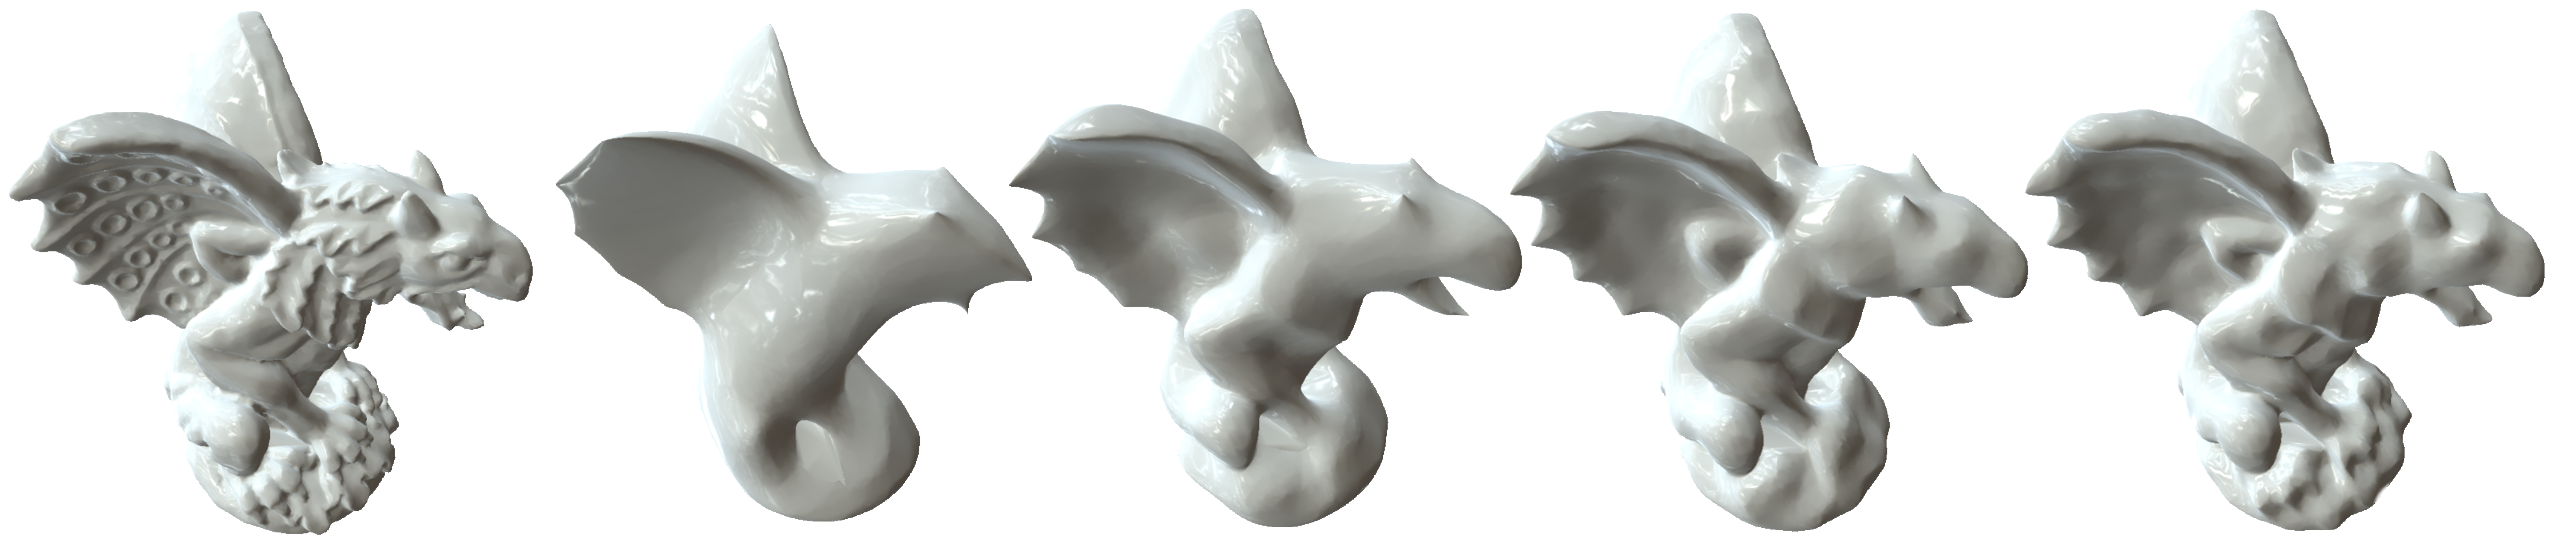
\includegraphics[width=1\textwidth]{img/Reconstructions_With_Eigenvectors}

\protect\caption{Mesh reconstruction with first $n$ eigenvectors of the Discrete Laplacian
Operator {[}Levy10{]}.}


\end{figure}


\end{frame}

\begin{frame}{Weights for Laplacian operator}


Desired property:

Non-negative weights $\omega_{ij}$ for $i\neq j$ ensure a positive
semi-definite matrix.
\begin{itemize}
\item Umbrella Operator $w_{ij}=\begin{cases}
1 & \,\,\,\mbox{if }j\in N\left(v_{i}\right)\\
0 & \,\,\,\mbox{else}
\end{cases}$
\item Fujiwara's Operator $w_{ij}=\begin{cases}
\frac{1}{\left\Vert v_{j}-v_{i}\right\Vert } & \,\,\,\mbox{if }j\in N\left(v_{i}\right)\\
0 & \,\,\,\mbox{else}
\end{cases}$
\end{itemize}

\note[item]{Fujiwara - {[}Desbrun99{]}}


\note[item]{Mean Value Coordinates - Floater03}


\note[item]{https://es.wikipedia.org/wiki/Matriz\_definida\_positiva}

\end{frame}

\begin{frame}{1999 Desbrun's operator for triangle meshes}


\framesubtitle{This operator only works with meshes composed only by \textbf{triangles}.}


\begin{center}
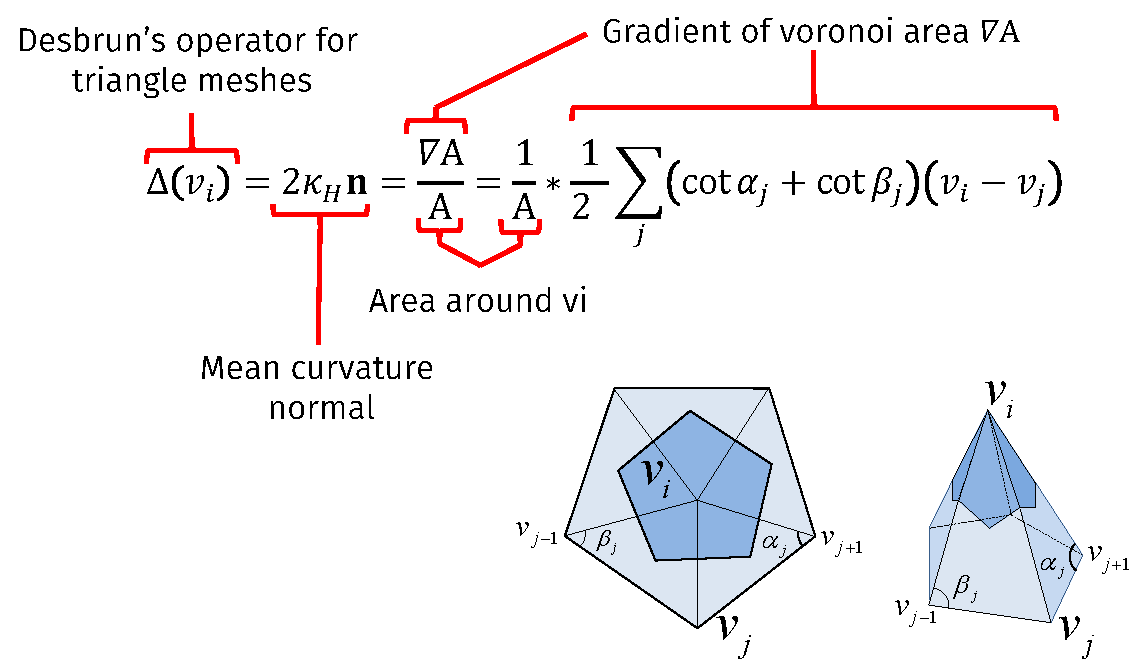
\includegraphics[width=0.9\columnwidth]{img/proposal_desbrun}
\par\end{center}

\end{frame}

\begin{frame}{2011 Xiong's MLBO operator for quad meshes}


\framesubtitle{This operator only work with meshes composed only by \textbf{quads}.}

\vspace{-10bp}

\begin{center}
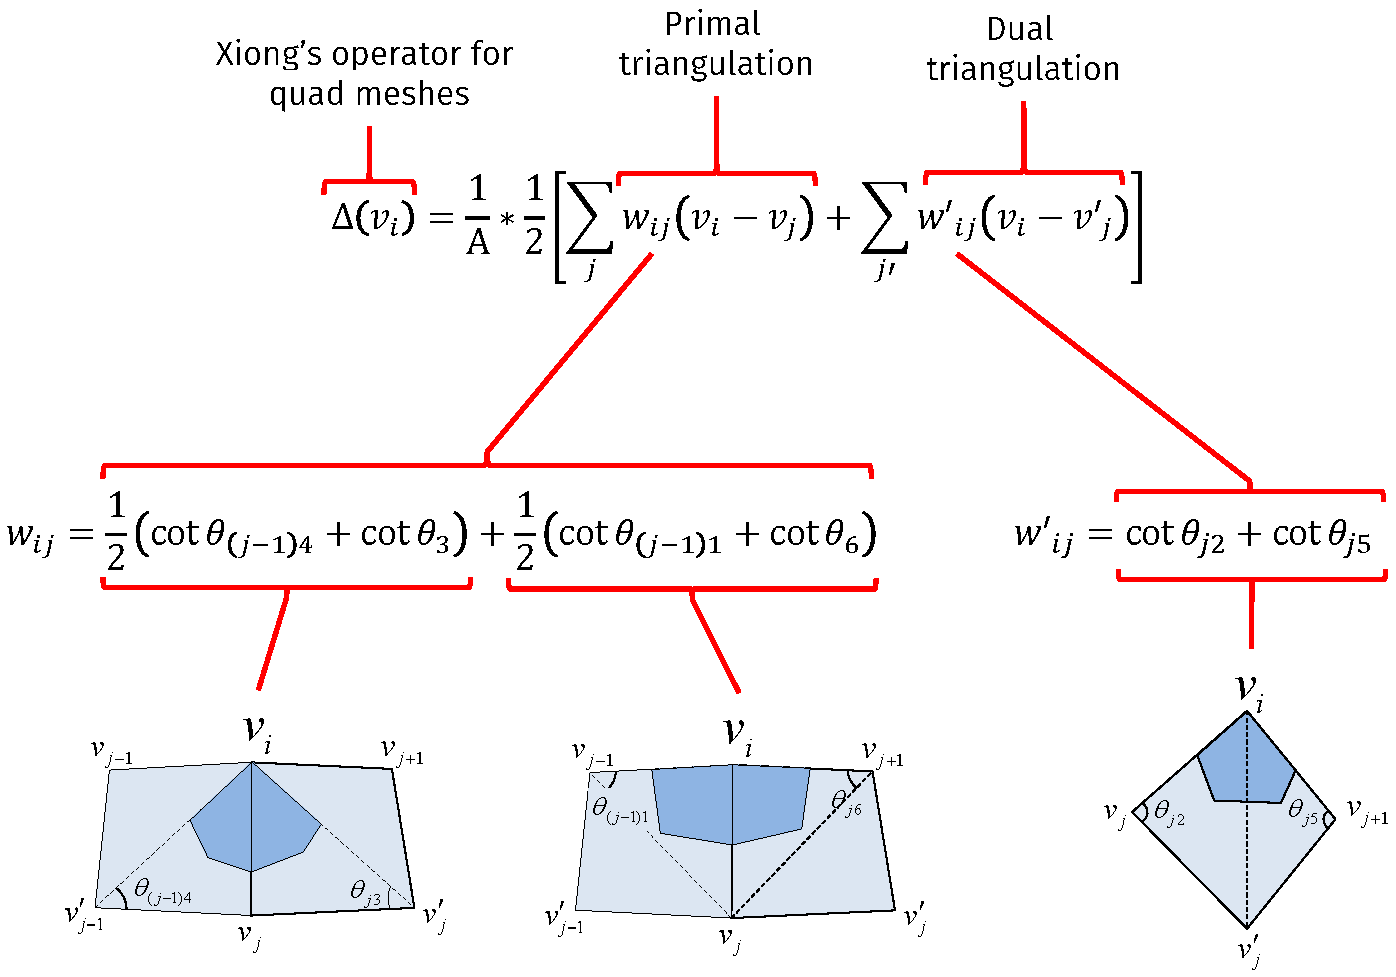
\includegraphics[width=1.0\columnwidth]{img/proposal_xiong}
\par\end{center}


\note[item]{where \textbf{$A_{i}$ }is the average area of the 1-ring neighborhood.}

\end{frame}

\begin{frame}{Laplacian applications on 3D modeling process}


\framesubtitle{General 3D modeling process on polygonal meshes.}


\begin{center}
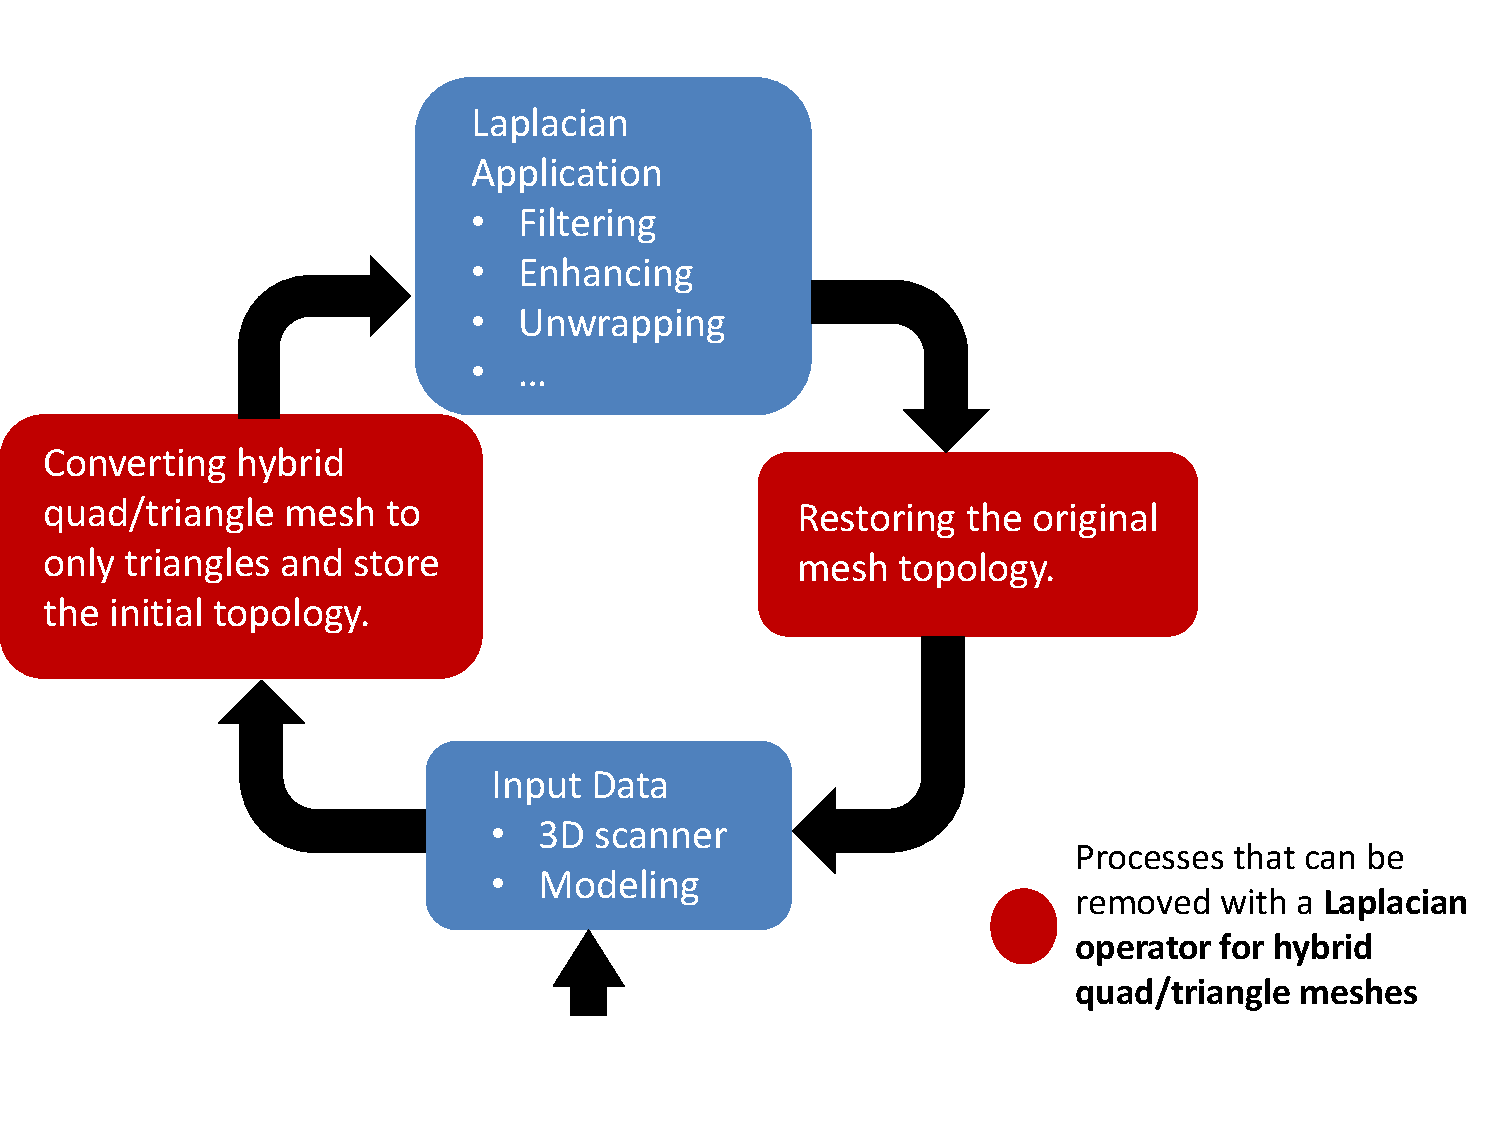
\includegraphics[bb=0bp 0bp 720bp 500bp,clip,width=0.95\textwidth]{img/ModelingProcess}
\par\end{center}

\end{frame}

\begin{frame}{Edge loops for faces}


Hybrid quad/triangle meshes are necessary to 3D modeling artists


\begin{center}
\begin{minipage}[c]{0.48\columnwidth}%
\begin{figure}
\begin{centering}
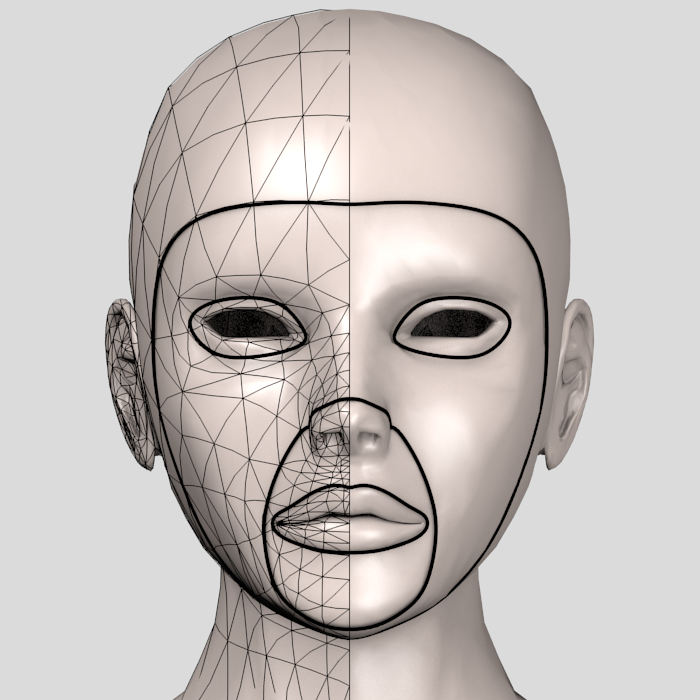
\includegraphics[width=1\columnwidth]{img/quad_faces2}
\par\end{centering}

\protect\caption{Triangle Mesh}
\end{figure}
%
\end{minipage}~%
\begin{minipage}[c]{0.48\columnwidth}%
\begin{figure}
\begin{centering}
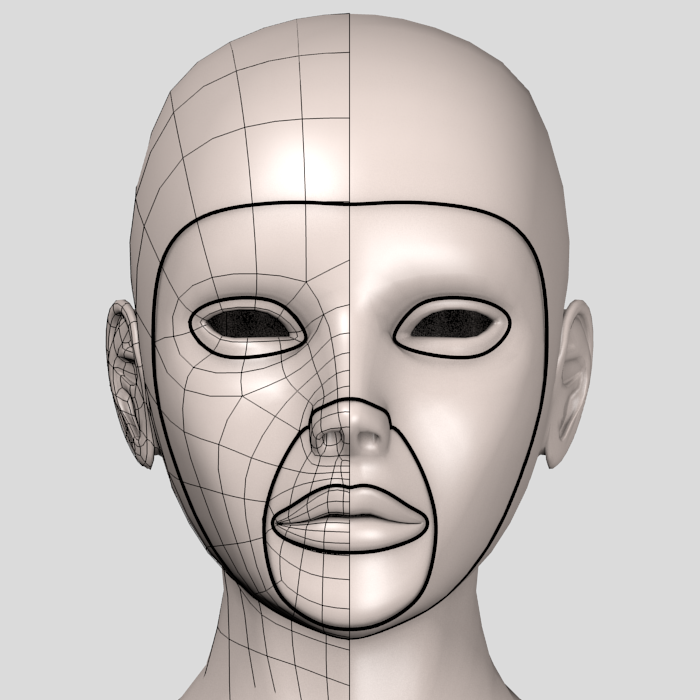
\includegraphics[width=1\columnwidth]{img/quad_faces}
\par\end{centering}

\protect\caption{Hybrid Quad/Triangle Mesh}
\end{figure}
%
\end{minipage}
\par\end{center}

\end{frame}

\section{Proposed Method}
\begin{frame}{Our proposal}


\begin{minipage}[c]{0.53\columnwidth}%
We propose an extension of the discrete Laplace-Beltrami operator
to work with hybrid quad/triangle meshes and eliminate the need of
triangulating the mesh and also allow the preservation of the original
topology.%
\end{minipage}~~%
\begin{minipage}[c]{0.43\columnwidth}%
\begin{center}
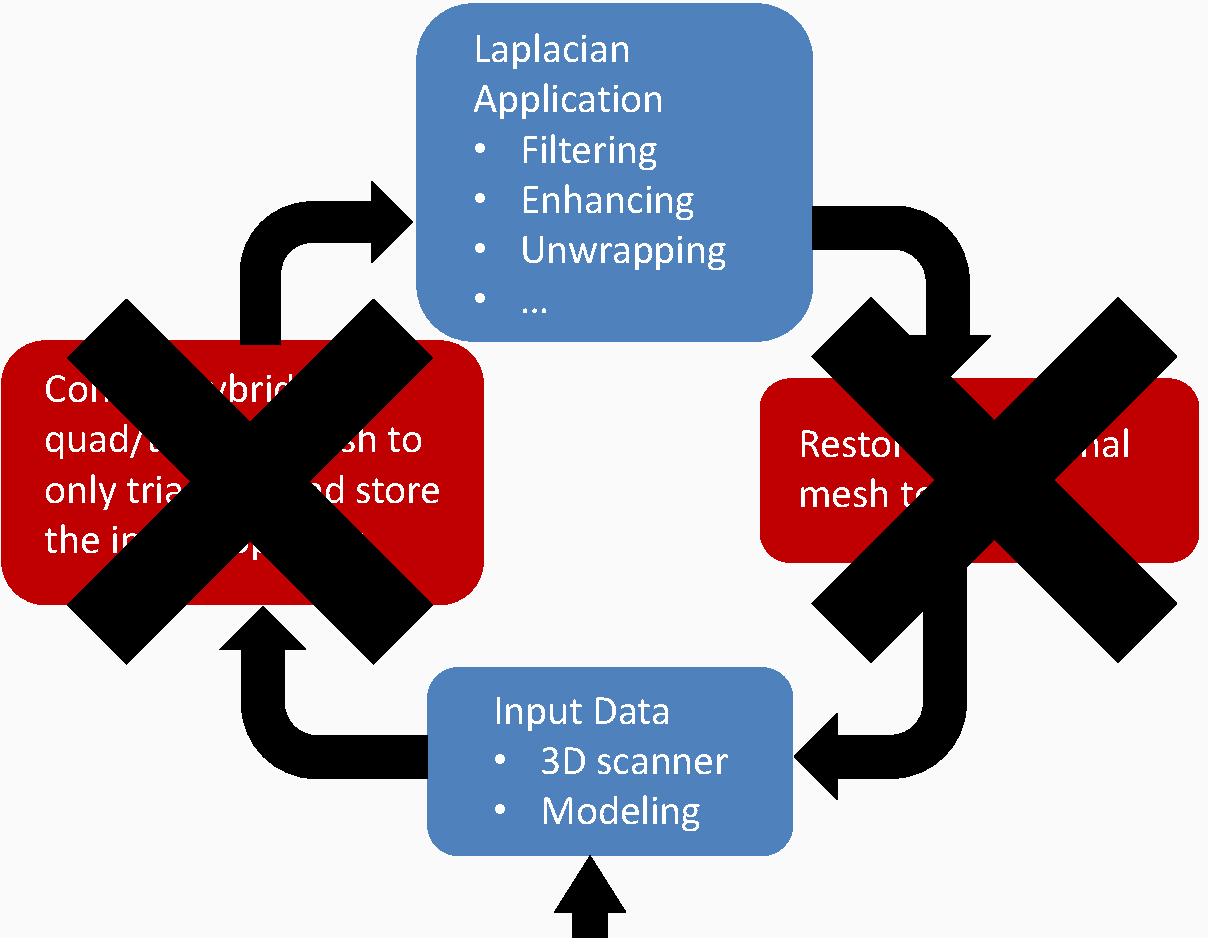
\includegraphics[width=1\columnwidth]{img/Our_Proposal_ModelingProcess}
\par\end{center}%
\end{minipage}


\end{frame}
 


\begin{frame}{Mathematical framework of our proposal}

 
\begin{center}
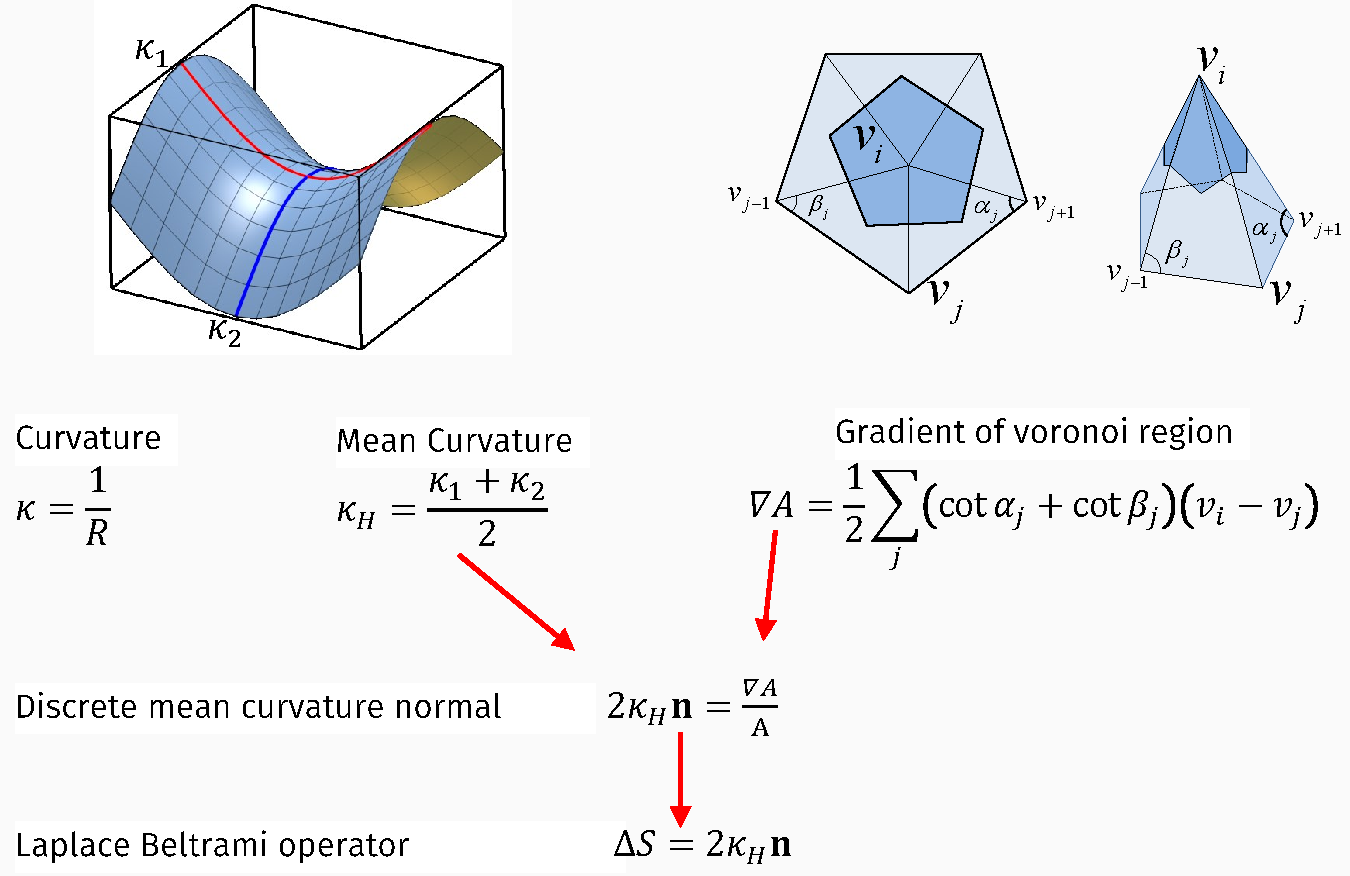
\includegraphics[width=1\textwidth]{img/proposal_kurvature}
\par\end{center}

\end{frame} 

\begin{frame}{Mathematical framework of our proposal}


\framesubtitle{Xiong's mean average area}


\begin{center}
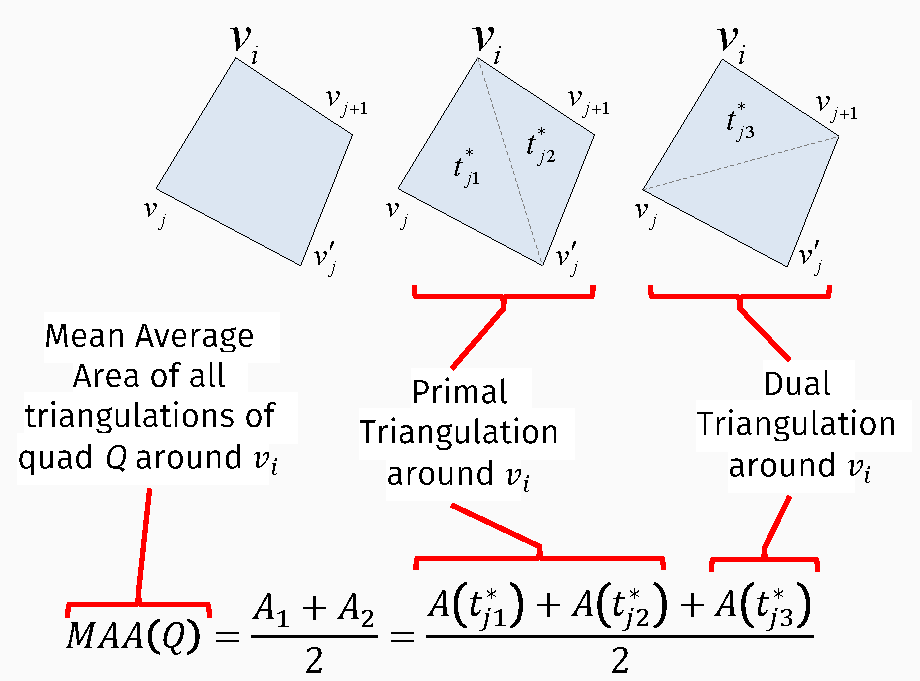
\includegraphics[width=0.8\textwidth]{img/proposal_maa}
\par\end{center}

\end{frame}

\begin{frame}{{\large{}Laplace Beltrami operator for hybrid quad/triangle meshes}}
\framesubtitle{Our proposal}



Area of hybrid region with quads $q_{j}$ and triangles $t_{k}$ around
$v_{i}$


\textrm{$A\left(v_{i}\right)=\underset{j=1}{\overset{m}{\sum}}A(q_{j})+\underset{k=1}{\overset{r}{\sum}}A(t_{k})$}


\bigskip{}



\pause{}


Applying Xiong's mean average area for quads


\textrm{$A\left(v_{i}\right)=\frac{1}{2}\underset{j=1}{\overset{m}{\sum}}\left[A\left(t_{j1}^{*}\right)+A\left(t_{j2}^{*}\right)+A\left(t_{j3}^{*}\right)\right]+\underset{k=1}{\overset{r}{\sum}}A(t_{k})$}


\bigskip{}



\pause{}


Applying Laplace operator


\textrm{$\Delta\left(v_{i}\right)=\frac{1}{2}\underset{j=1}{\overset{m}{\sum}}\left[\Delta\left(t_{j1}^{*}\right)+\Delta\left(t_{j2}^{*}\right)+\Delta\left(t_{j3}^{*}\right)\right]+\underset{k=1}{\overset{r}{\sum}}\Delta(t_{k})$}


\bigskip{}



\pause{}


Rewriting $\Delta\left(v_{i}\right)$ we define the \textbf{\textsl{Triangle
Quad Laplace Beltrami Operator}}


\textrm{$\Delta\left(v_{i}\right)=\frac{1}{2A_{i}}\underset{j=1}{\overset{m}{\sum}}w_{ij}\left(v_{j}-v_{i}\right)$}


\end{frame}

\begin{frame}{Weights for TQLBO - Our proposal}


\framesubtitle{{\small{}The 5 basic triangle-quad cases with a vertex $V_{i}$
and the relationship with $V_{j}$ and $V_{j}^{\prime}$}}


\vspace{-10bp}



\hspace{10bp}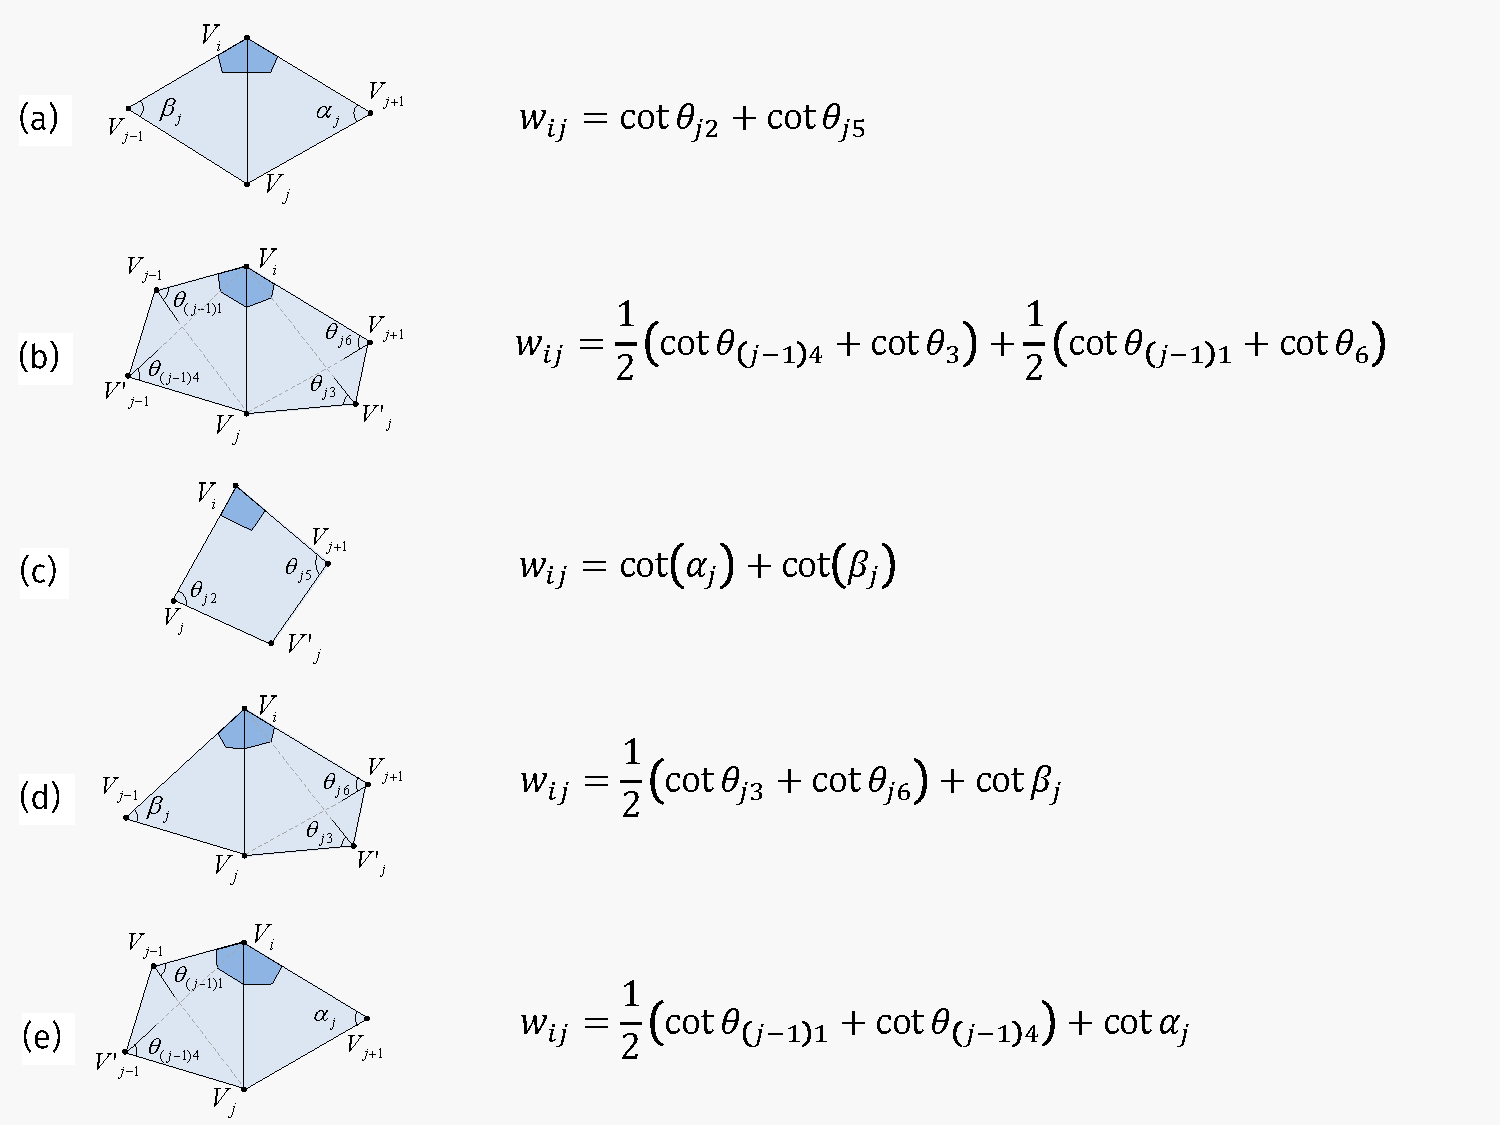
\includegraphics[width=0.85\paperwidth]{img/proposal_weights}

\end{frame}

\begin{frame}{Laplace operator as a matrix equation}
\framesubtitle{Our proposal}


We define a TQLBO as a matrix equation


\begin{equation}
L\left(i,j\right)=\begin{cases}
-\frac{1}{2A_{i}}w_{ij} & \mbox{if }j\in N\left(v_{i}\right)\\
\frac{1}{2A_{i}}\underset{k\in N\left(v_{i}\right)}{\sum}w_{ik} & \mbox{if }i=j\\
0 & \mbox{otherwise}
\end{cases}\label{eq:TQLBO_Laplacian_Matrix}
\end{equation}



Where $L$ is an $n\times n$ matrix, $n$ is the number of vertices
, $N\left(v_{i}\right)$ is the 1-ring neighborhood with shared face
to $v_{i}$, $A_{i}$ is the ring area around $v_{i}$.

\end{frame}



\section{Evaluation and Results}
\begin{frame}{Enhancing}


A standard diffusion process is used.


\begin{center}
$\ensuremath{\frac{\partial V}{\partial t}=\lambda L\left(V\right)}$
\par\end{center}


To solve this equation, implicit integration is used as well as a
normalized version of TQLBO matrix


\begin{center}
$\left(I-\left|\lambda dt\right|W_{p}L\right)V^{\prime}=V^{t}$
\par\end{center}


\begin{center}
$\ensuremath{V^{t+1}=V^{t}+\mbox{sign}\left(\lambda\right)\left(V^{\prime}-V^{t}\right)}$
\par\end{center}


where $L$ is the TQLBO, $V^{\prime}$ are the smoothing vertices,
$V^{t}$ are the actual vertices positions, $W_{p}$ is a diagonal
matrix with vertex weights, and $\lambda dt$ is the inflate factor.

\end{frame}

\begin{frame}{Sculpting with enhancing filter}


\framesubtitle{Inflate Brush}


Real-time brushes require the Laplacian matrix be constructed with
the vertices that are within the sphere radius defined by the user,
reducing the matrix to be processed.


\begin{center}
$L\left(i,j\right)=\begin{cases}
-\frac{w_{ij}}{\underset{j\in N\left(v_{i}\right)}{\sum}w_{ij}} & \mbox{if }\left\Vert v_{i}-u\right\Vert <r\wedge\left\Vert v_{j}-u\right\Vert <r\\
0 & \mbox{if }\left\Vert v_{i}-u\right\Vert <r\wedge\left\Vert v_{j}-u\right\Vert \geq r\\
\delta_{ij} & \mbox{otherwise}
\end{cases}$
\par\end{center}


Where $v_{j}\in N\left(v_{i}\right)$, $u$ is the sphere center of
radius $r$. The matrices should remove rows and columns of vertices
that are not within the radius.

\end{frame}

\begin{frame}{Compute the minimal surface with TQLBO results}


\begin{figure}
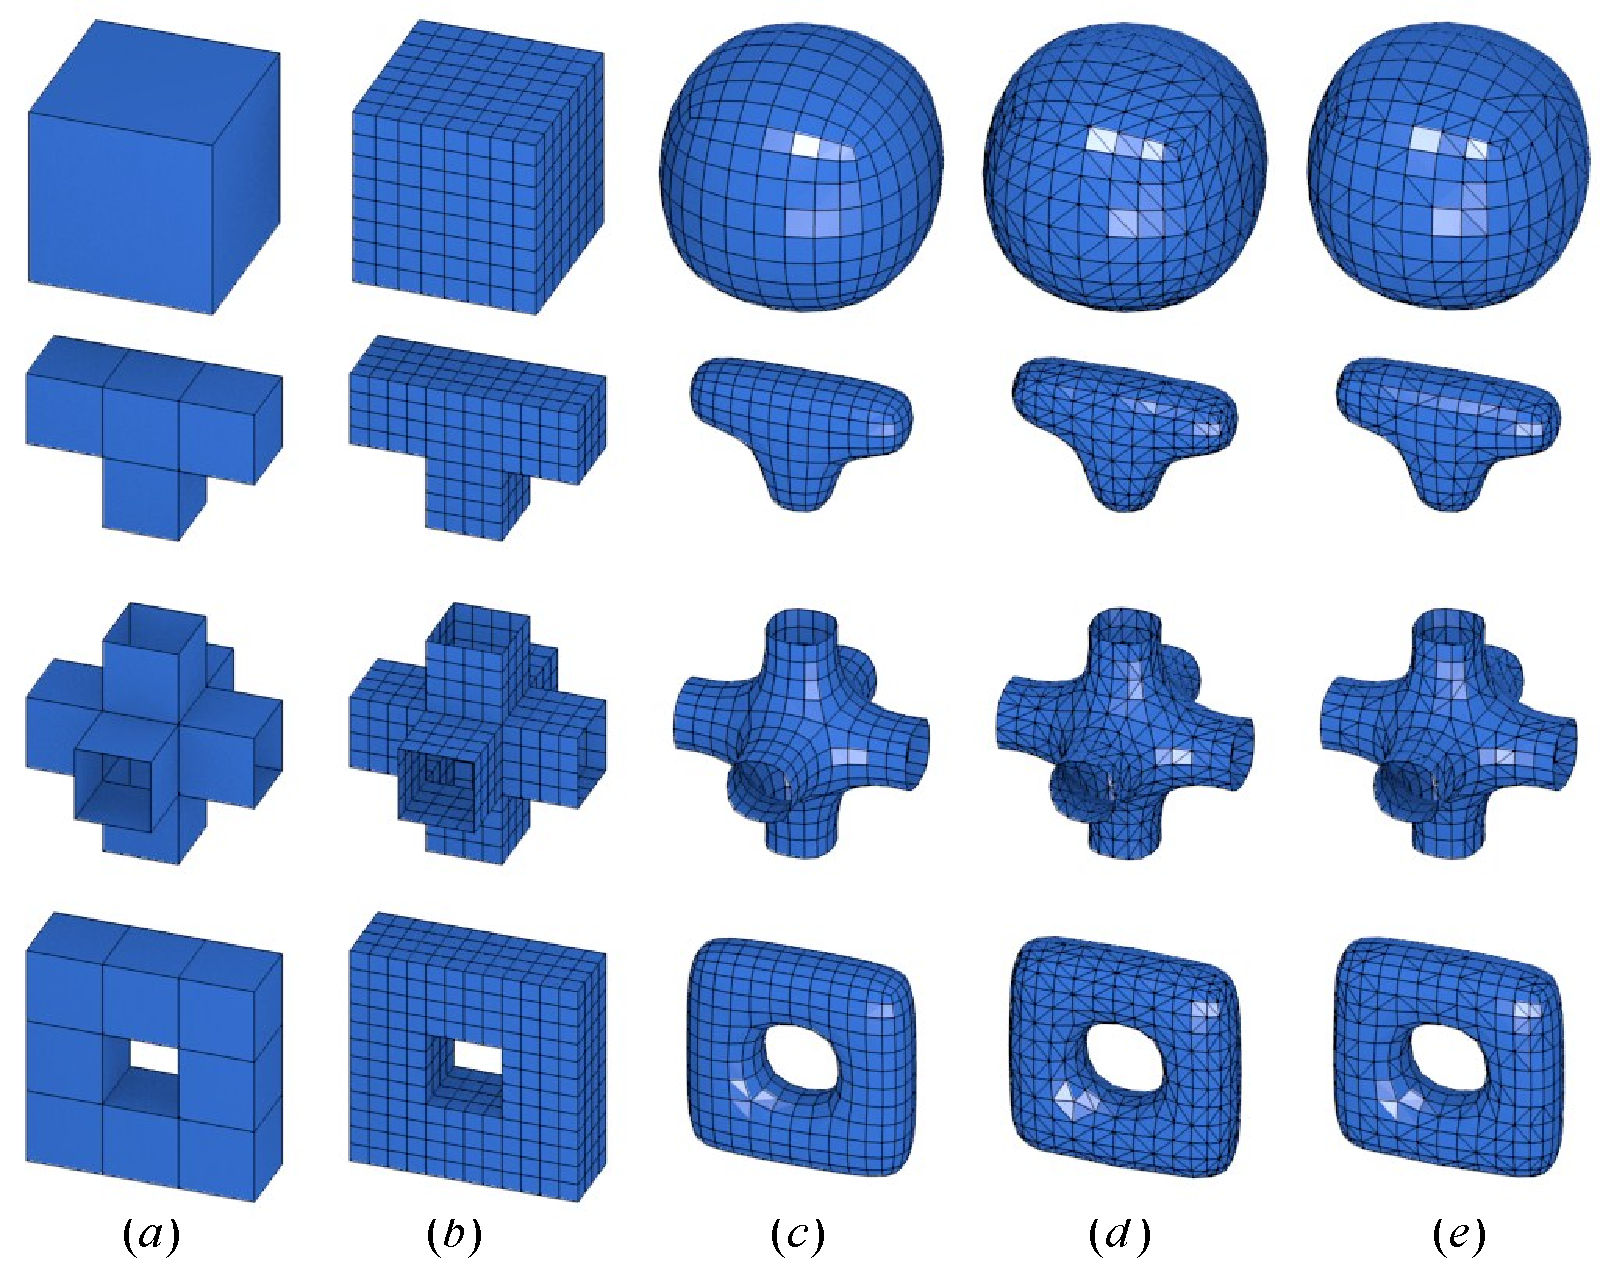
\includegraphics[height=0.6\paperheight]{img/test_triangles_quads}

\protect\caption{(a) Original Model. (b) Simple subdivision. (c), (d) (e) Laplacian
smoothing with $\lambda=7$ and 2 iterations: (c) for quads, (d) for
triangles, (e) for triangles and quads randomly chosen.}


\end{figure}


\end{frame}

\begin{frame}{Shape Inflation with enhancing filter results}


\begin{figure}
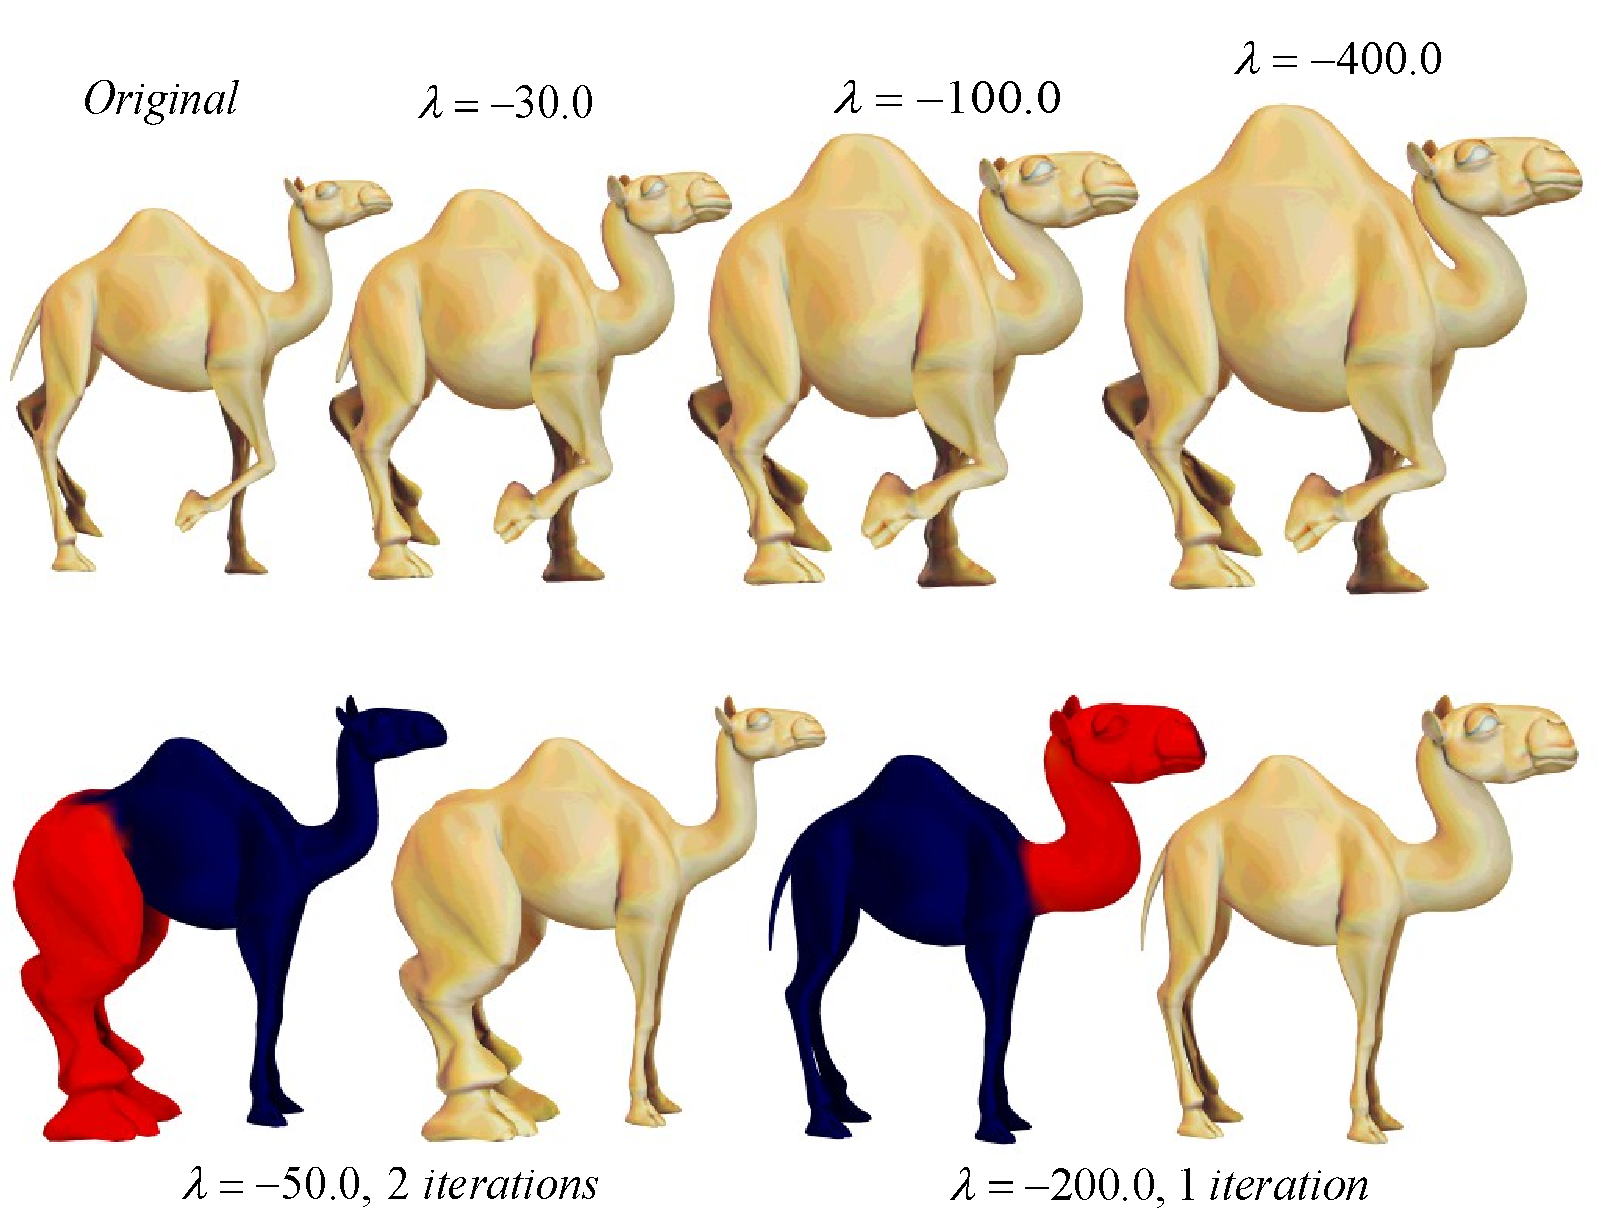
\includegraphics[height=0.5\textwidth]{img/camello_enhanced2}

\protect\caption{Top row: Original camel model on left. Shape inflation with $\lambda=-30.0$,
$\lambda=-100.0$, $\lambda=-400.0$. Bottom row: Shape inflation
with weight vertex group, $\lambda=-50.0$ and 2 iterations for the
legs, $\lambda=-200.0$ and 1 iteration for head and neck.}


\end{figure}


\end{frame}

\begin{frame}{Inflate brush results}


\begin{figure}
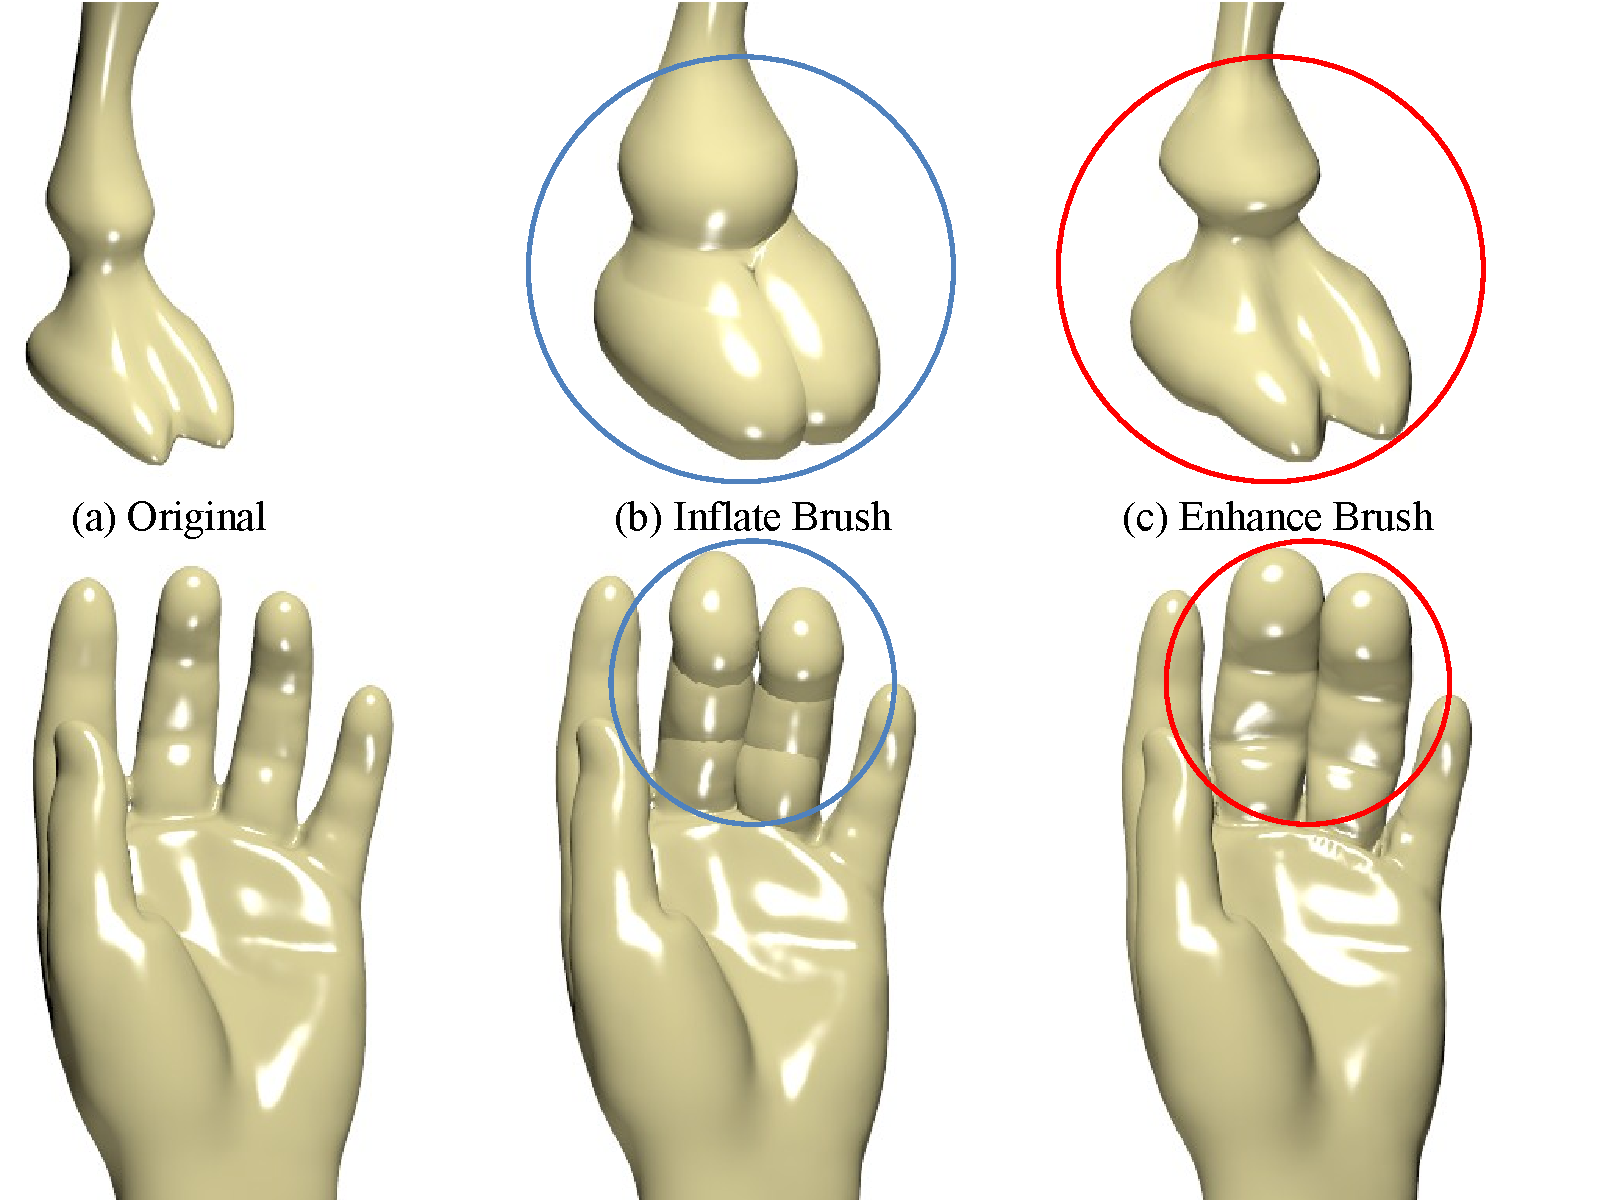
\includegraphics[height=0.5\textwidth]{img/sculpt_brush}

\protect\caption{Top row: (a) Leg Camel, (b) Traditional inflate brush for leg into
blue circle, (c) Shape inflation brush for leg into red circle. Bottom
row: (a) Hand, (b) Traditional inflate brush for fingers into blue
circle, (c) Shape inflation brush for fingers in red circle.}


\end{figure}


\end{frame}



\begin{frame}{Inflate brush performance}


\vspace{-10bp}


\begin{figure}
\hspace{-20bp}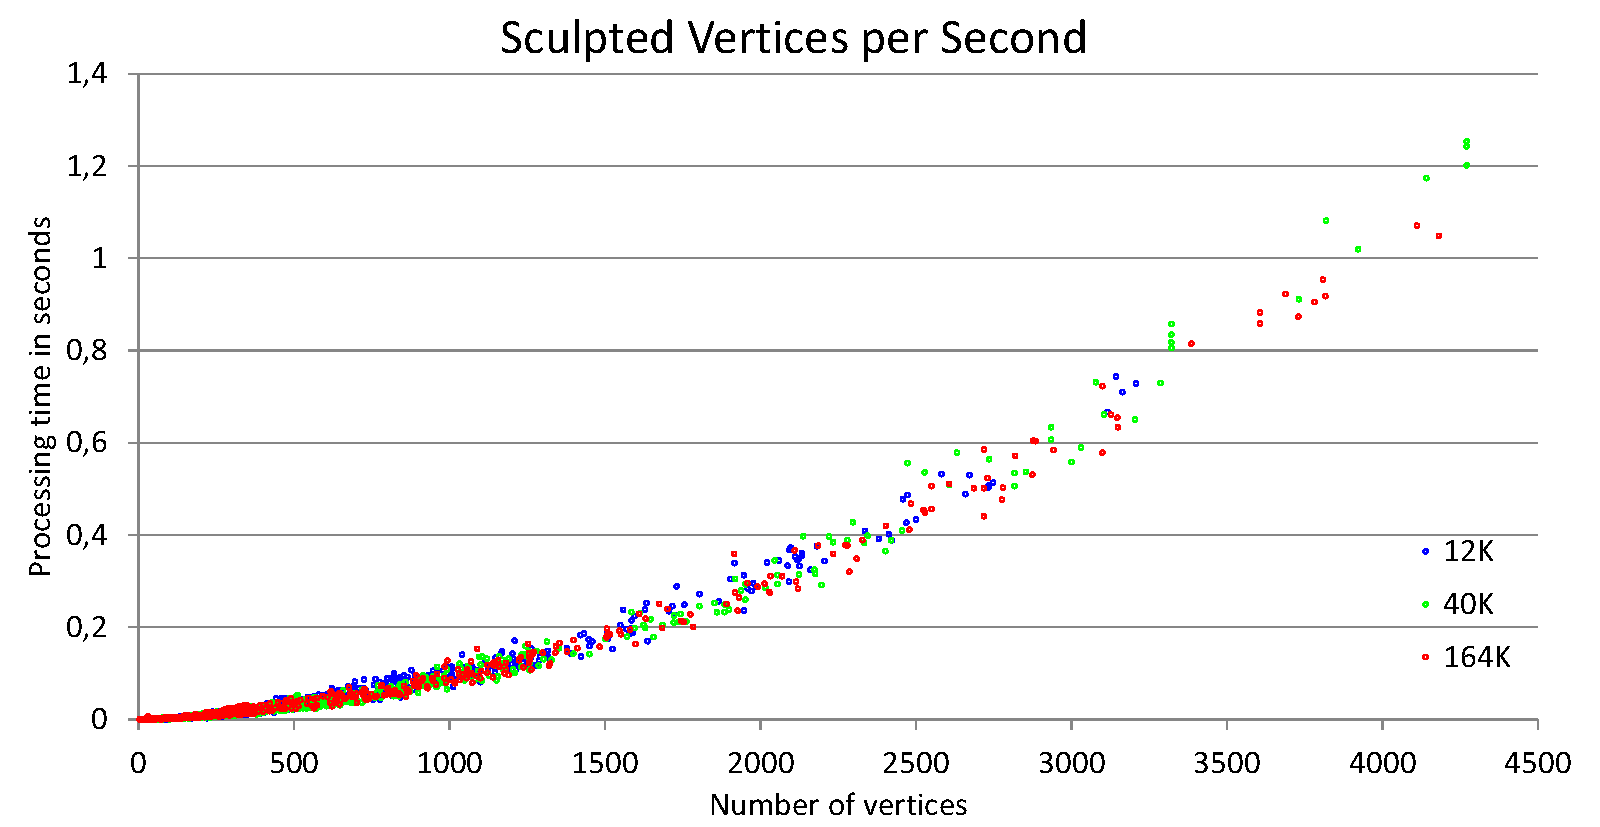
\includegraphics[height=0.7\textheight]{img/verts_per_second_sculpt}

\protect\caption{Performance of our dynamic shape inflation brush in terms of the sculpted
vertices per second. Three models with 12K, 40K, 164K vertices used
for sculpting in real time.}


\end{figure}


\end{frame}


\section{Products}
\begin{frame}{1st product - Conference paper}


\framesubtitle{{\small{}Brazilian Symposium on Computer Graphics and Image Processing
SIBGRAPI 2013}}


\begin{center}
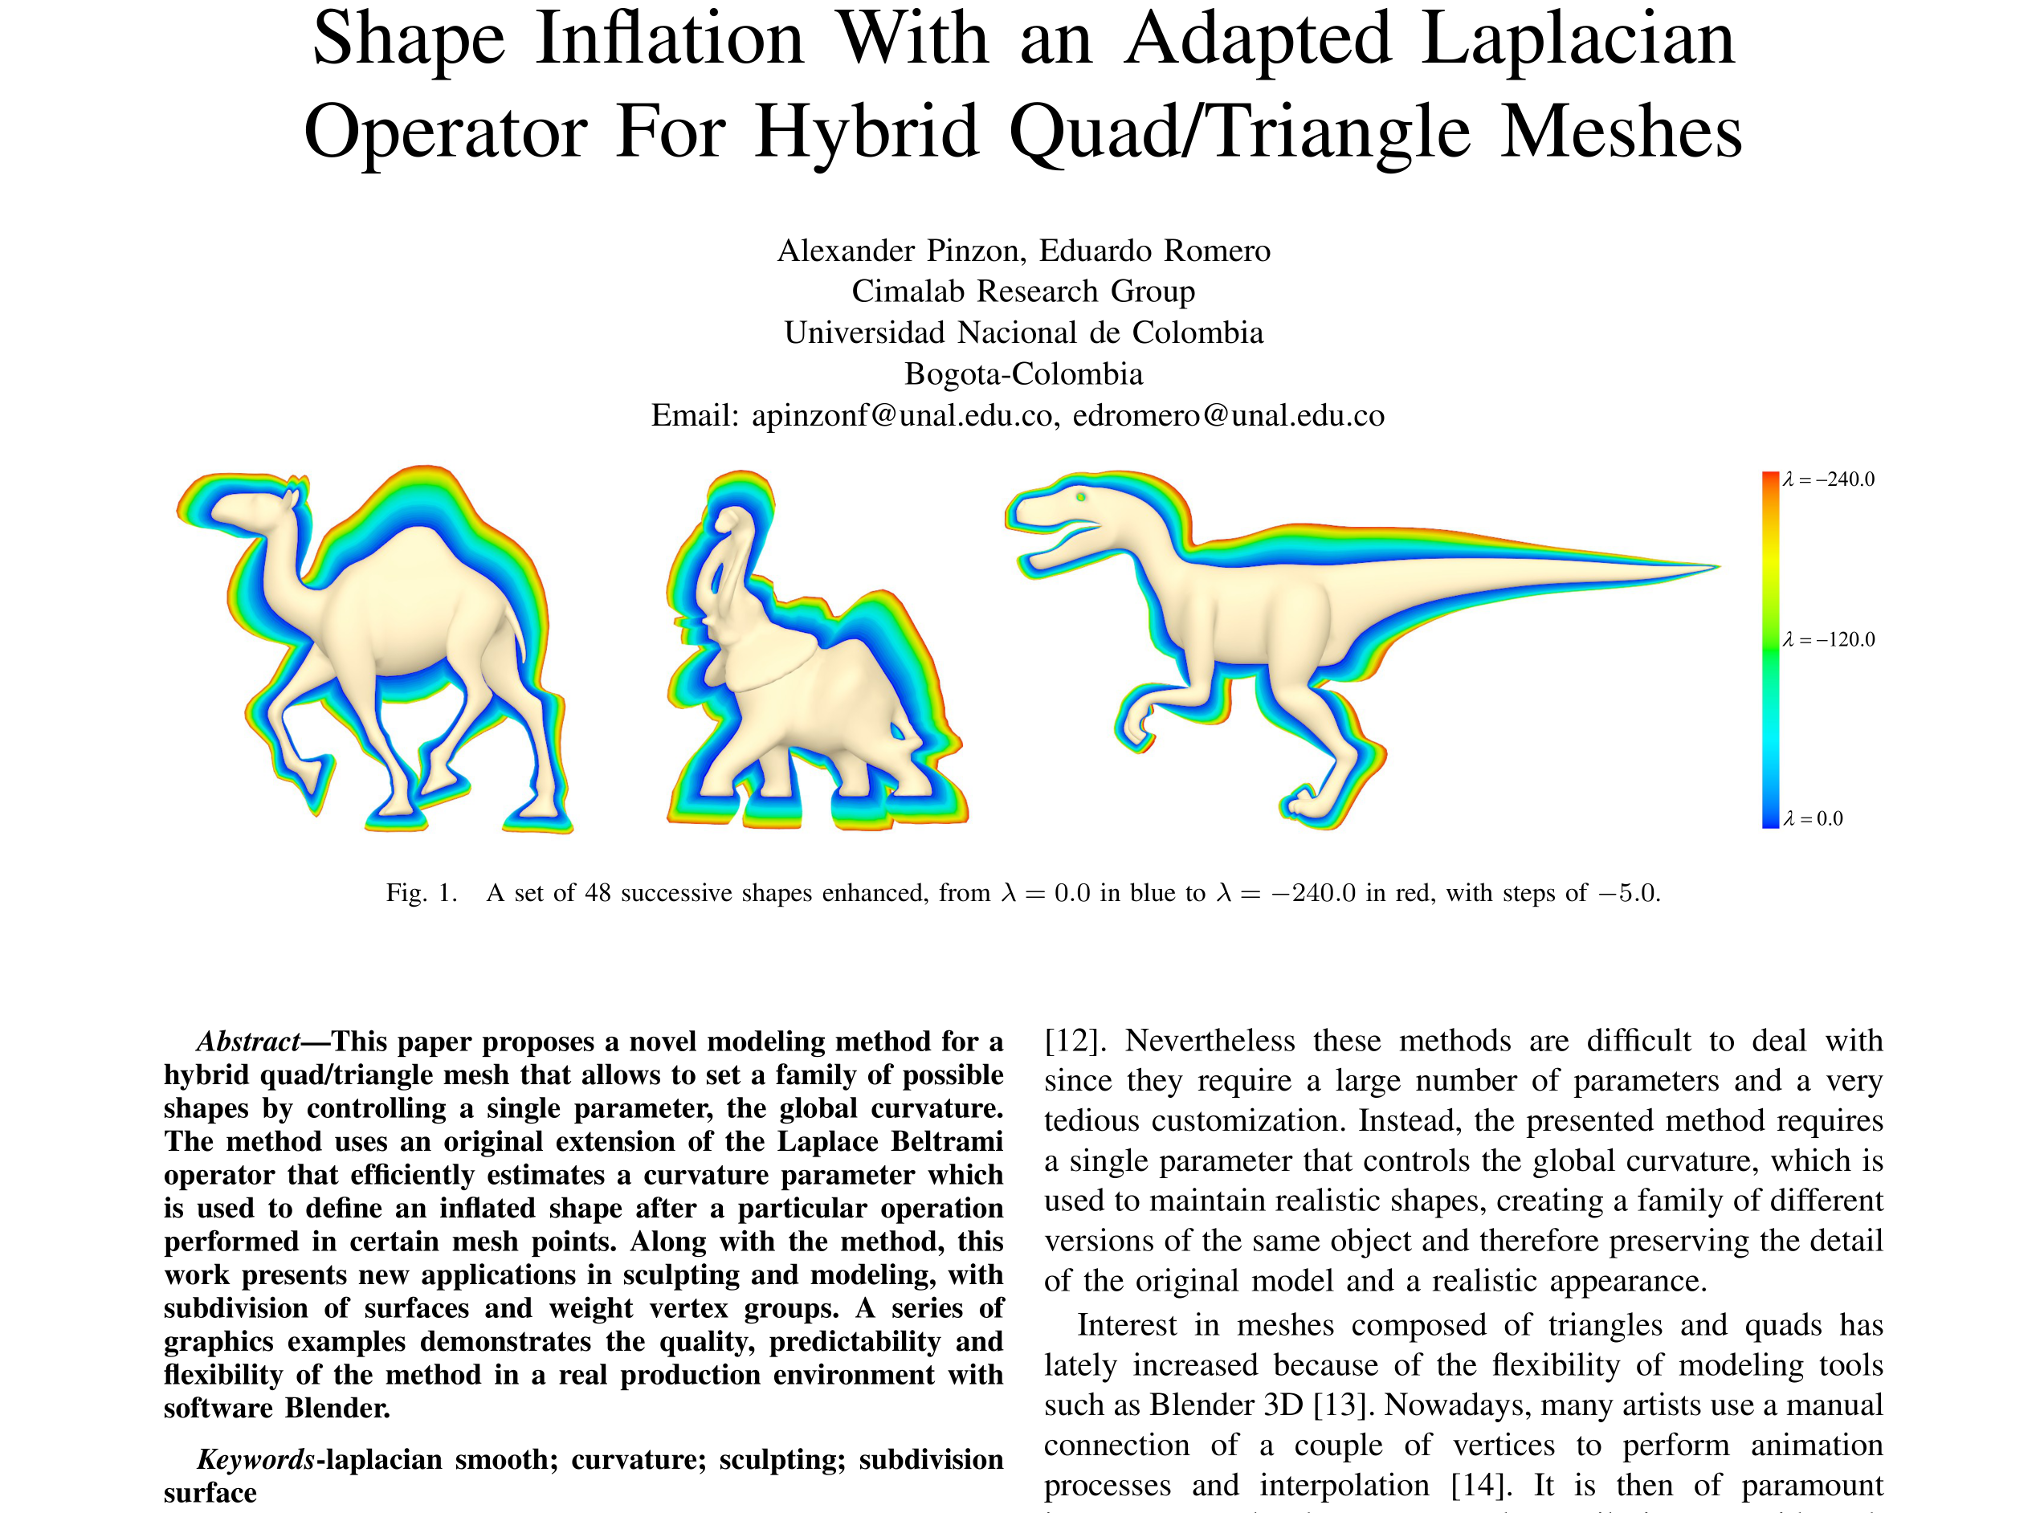
\includegraphics[height=0.8\textheight]{img/PaperTQLBO3}
\par\end{center}

\end{frame}

\begin{frame}{2nd product - Awarded internship}


\framesubtitle{Mesh smoothing based on curvature flow operator in a diffusion equation}
\begin{description}
\item [{Sponsor:}] Google Inc - Google Summer of Code 2012 program
\item [{Project:}] Mesh smoothing based on curvature flow operator in a
diffusion equation
\item [{Synopsis:}] This project proposes a new and robust mesh smoothing
tool that removes the noise on the surfaces of models captured with
3d scanners, zcameras among others.
\item [{Blender:}] This software is an open source 3D application for modeling,
rendering, composing, video editing and game creation.
\end{description}
\end{frame}

\begin{frame}{2nd Prod - Laplacian smooth tool for Blender}


\framesubtitle{Mesh smoothing based on curvature flow operator in a diffusion equation}


We define a Laplacian matrix for mesh smoothing with support for hybrid
quad/triangle meshes with holes as


\begin{center}
$L(i,j)=\begin{cases}
-\frac{1}{2A_{i}}w_{ij} & \mbox{if }j\in N(v_{i})\wedge v_{i}\notin\mbox{Boundary}\\
\frac{1}{2A_{i}}\underset{j\in N\left(v_{i}\right)}{\sum}w_{ij} & \mbox{if }i=j\wedge v_{i}\notin\mbox{Boundary}\\
-\frac{1}{\left\Vert v_{i}-v_{j}\right\Vert } & \mbox{if }j\in N(v_{i})\wedge\left\{ v_{i},v_{j}\right\} \in\mbox{Boundary}\\
\frac{2}{E_{i}}\underset{j\in N\left(v_{i}\right)}{\sum}\frac{1}{\left\Vert v_{i}-v_{j}\right\Vert } & \mbox{if }i=j\wedge\left\{ v_{i},v_{j}\right\} \in\mbox{Boundary}\\
0 & \mbox{otherwise}
\end{cases}$
\par\end{center}


$w_{ij}$ is the TQLBO defined in equation (\ref{eq:TQLBO_Laplacian_Matrix})


$E_{i}=\underset{j\in N\left(v_{i}\right)}{\sum}e_{ij}$ .

\end{frame}

\begin{frame}{2nd Product - User interface}


\framesubtitle{Mesh smoothing based on curvature flow operator in a diffusion equation}


\begin{figure}[H]
\noindent \begin{centering}
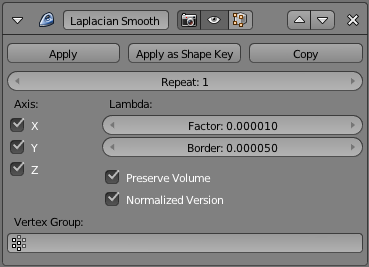
\includegraphics[width=0.7\columnwidth]{img/Apinzonf_Diagram_Modifier_Panel}
\par\end{centering}

\protect\caption{Panel inside blender user interface of the Laplacian Smooth modifier
tool.}
\end{figure}


\end{frame}

\begin{frame}{2nd Product - Results}


\framesubtitle{Mesh smoothing based on curvature flow operator in a diffusion equation}


\begin{figure}[H]
\noindent \begin{centering}
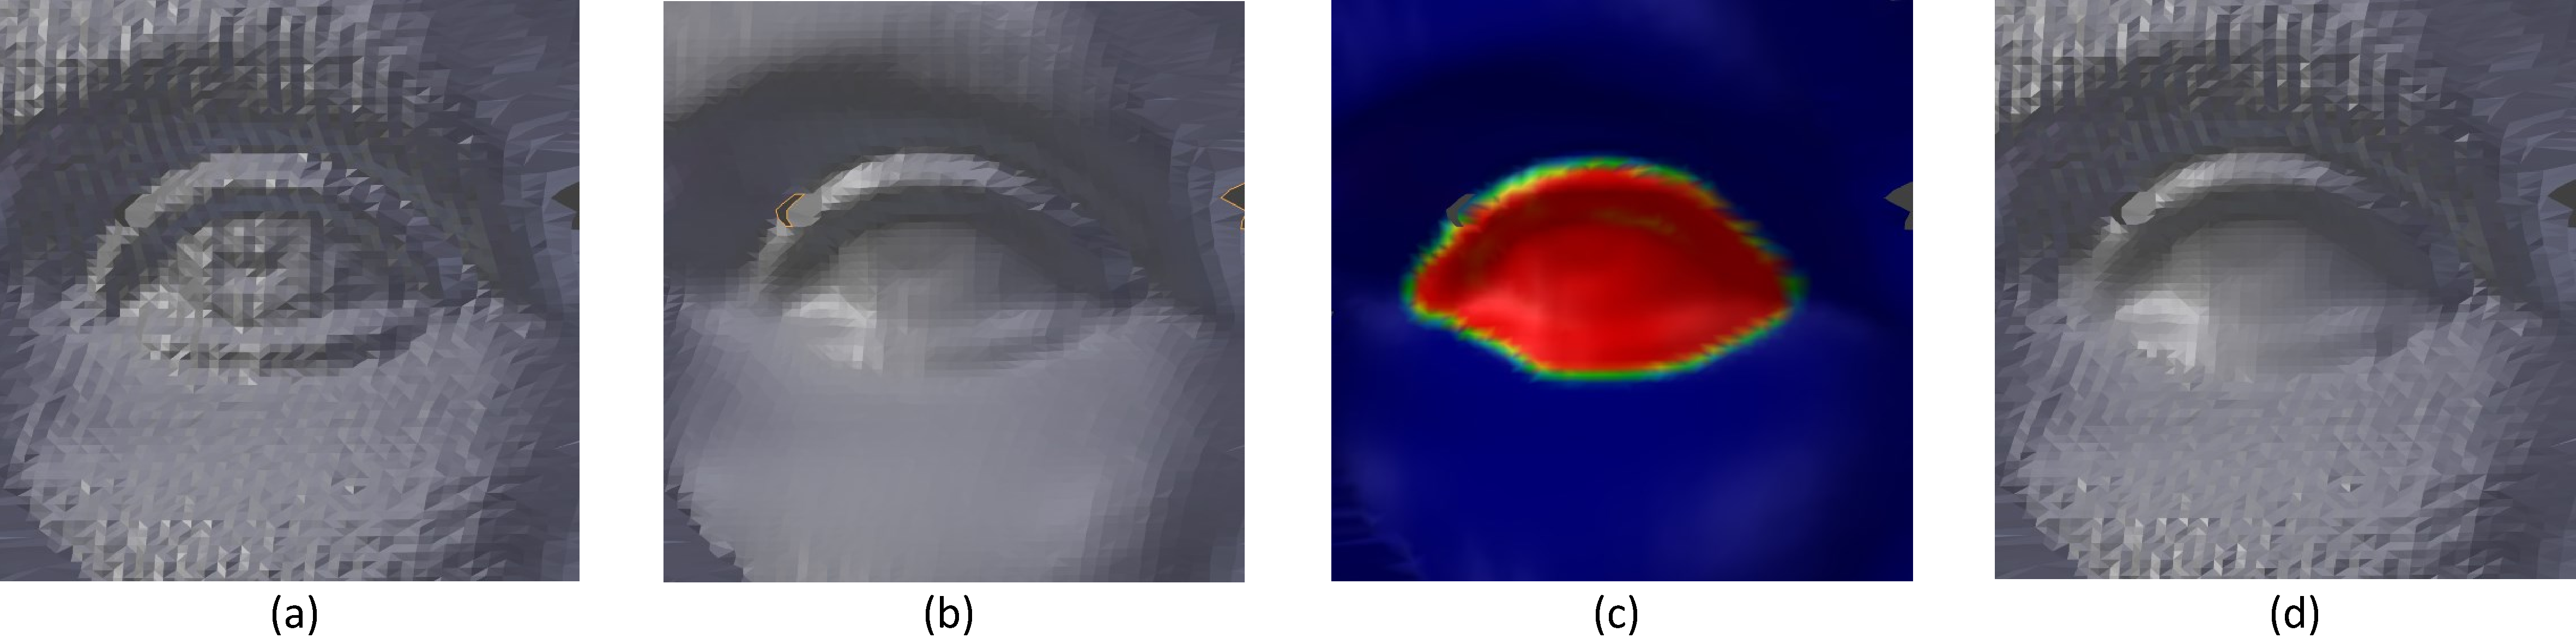
\includegraphics[width=1\textwidth]{img/LaplacianSmoothingVertecGroup}
\par\end{centering}

\protect\caption{Use of weights per vertex to constrain the effect of mesh smoothing.
(a) Original Model. (b) Smoothing with $\lambda=1.5$. (c) Red vertices
$weight=1.0$, blue vertices $weight=0.0$. (d) Smoothing with $\lambda=2.5$.
 Red vertices were the only vertices smoothed.}
\end{figure}


\end{frame}



\begin{frame}{2nd Product - Results}


\framesubtitle{Mesh smoothing based on curvature flow operator in a diffusion equation}


\begin{figure}[H]
\noindent \begin{centering}
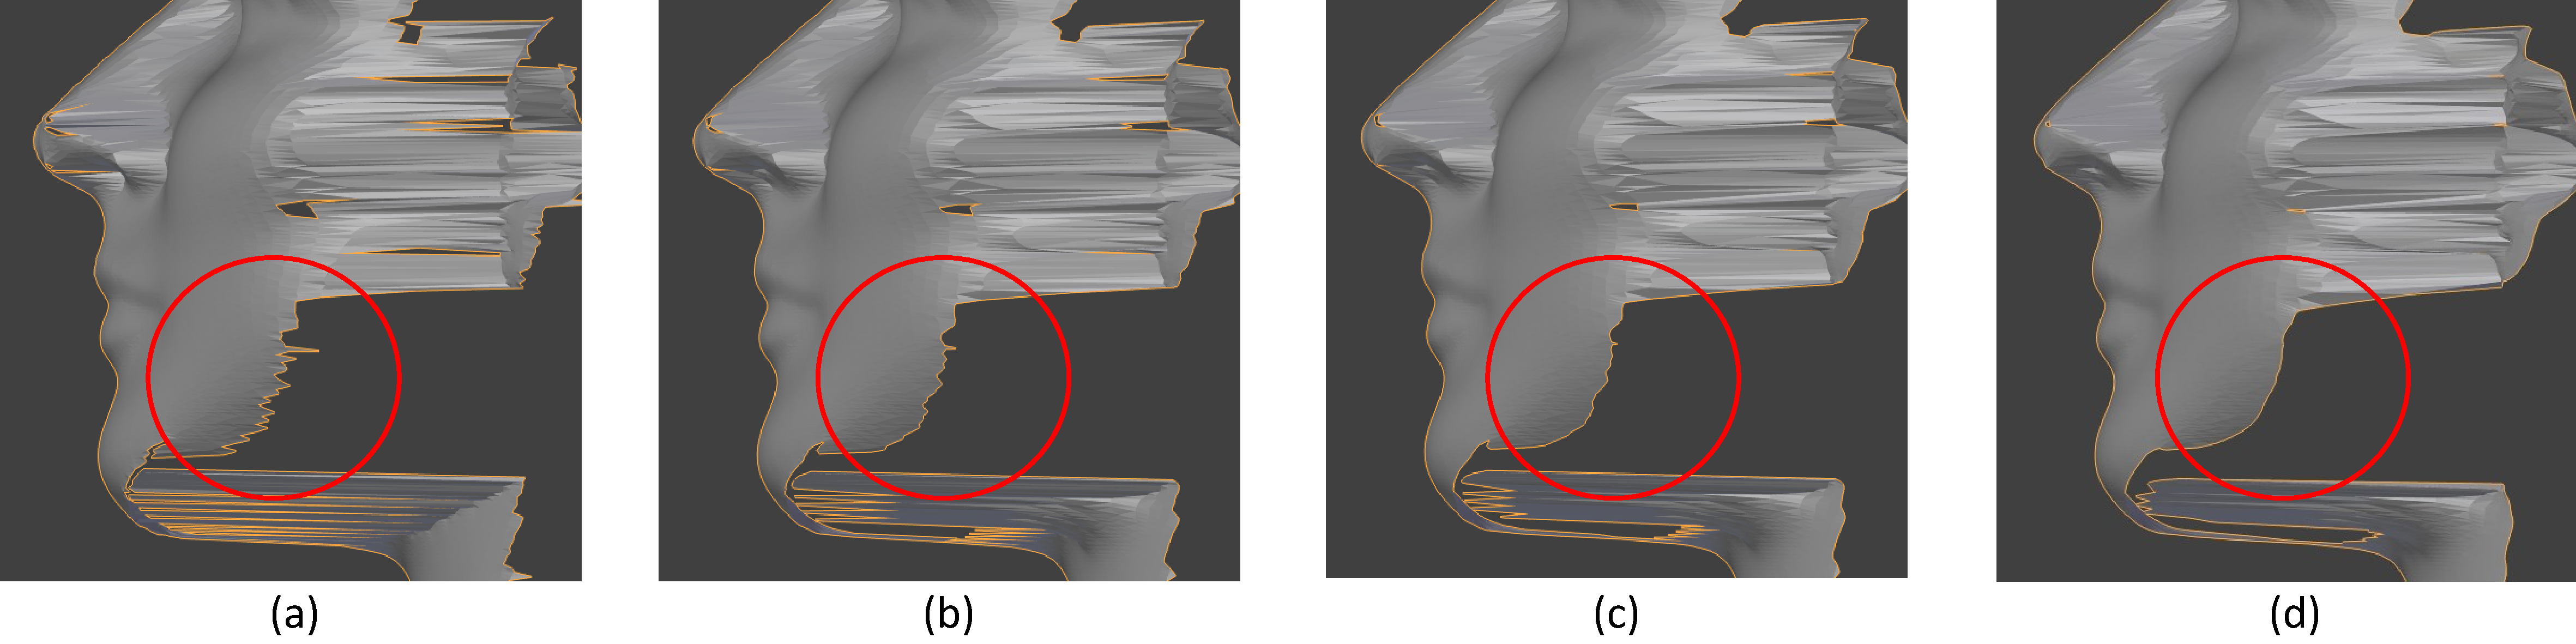
\includegraphics[width=1\textwidth]{img/LaplacianSmoothingBoundary}
\par\end{centering}

\protect\caption{Smoothing boundary changing $\lambda_{Border}$ factor. (a) Original
Model. (b) Smoothing $\lambda_{Border}=1.0$. (c) Smoothing $\lambda_{Border}=2.5$
(d) Smoothing with $\lambda_{Border}=10.0$. }
\end{figure}
 

\end{frame}
 
\begin{frame}{3rd product - Awarded internship}


\framesubtitle{Mesh Editing with Laplacian Deform}
\begin{description}
\item [{Sponsor:}] Google Inc - Google Summer of Code 2013 program
\item [{Project:}] Mesh Editing with Laplacian Deform
\item [{Synopsis:}] This project proposes a new tool that allows to pose
a mesh while preserving geometric details of the surface.
\item [{Blender:}] This software is an open source 3D application for modeling,
rendering, composing, video editing and game creation.
\end{description}
\end{frame}

 
\begin{frame}{3rd product - Differential coordinates}


\framesubtitle{Mesh Editing with Laplacian Deform}


\begin{equation}
\delta_{i}=\overset{m}{\underset{j=1}{\sum}}w_{ij}\left(v_{i}-v_{j}\right)\label{eq:DifferentialCoordinate}
\end{equation}



\begin{figure}[H]
\noindent \begin{centering}
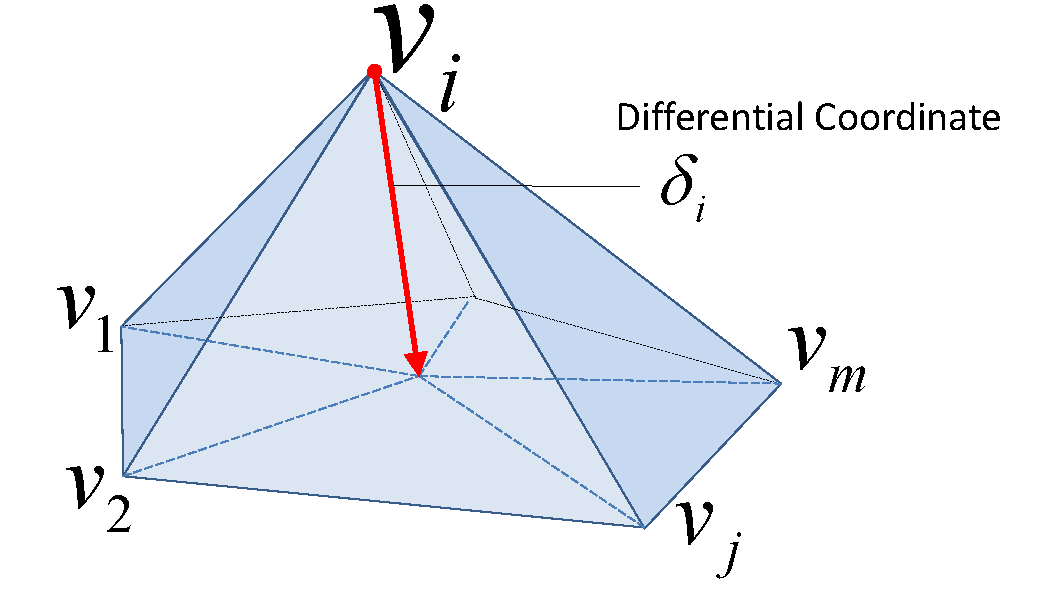
\includegraphics[width=0.4\columnwidth]{img/DifferentialCoordinates}
\par\end{centering}

\protect\caption{Difference between $v_{i}$ and the center of mass of its neighbors
$v_{1},...,v_{m}$.}
\end{figure}



$w_{ij}$ is the TQLBO defined in equation (\ref{eq:TQLBO_Laplacian_Matrix})

\end{frame}

\begin{frame}{3rd product - Laplacian deform}


\framesubtitle{Mesh Editing with Laplacian Deform}


The linear system for finding the new pose of a mesh is


\begin{equation}
\begin{bmatrix}L\\
W_{c}
\end{bmatrix}V=\begin{bmatrix}\delta\\
W_{c}C
\end{bmatrix}\label{eq:LaplacianDefomSystem}
\end{equation}

\begin{description}
\item [{$L$}] is a matrix that used our TQLBO defined in equation (\ref{eq:TQLBO_Laplacian_Matrix}). 
\item [{$Wc$}] is a matrix that has only ones in the indices of anchor
vertices. 
\item [{$V$}] is a vector with the vertices of the mesh positions.
\item [{$C$}] is a vector with coordinates of anchor vertices after several
manual transformations. 
\item [{$\delta$}] is the differential coordinates defined in equation
\textrm{(\ref{eq:DifferentialCoordinate}).}
\end{description}
\end{frame}

\begin{frame}{3rd product - User interface}


\framesubtitle{Mesh Editing with Laplacian Deform}


\noindent \begin{center}
\begin{figure}[H]
\noindent \begin{centering}
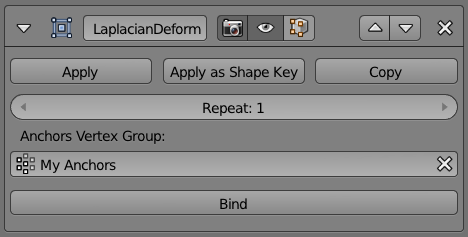
\includegraphics[width=0.7\columnwidth]{img/Apinzonf_Diagram_Deform_Modifier_Panel_01}
\par\end{centering}

\protect\caption{Panel inside Blender user interface of the Laplacian Deform modifier
tool.}
\end{figure}

\par\end{center}

\end{frame}



\begin{frame}{3rd product - Results}


\framesubtitle{Mesh Editing with Laplacian Deform}


\begin{figure}[H]
\noindent \begin{centering}
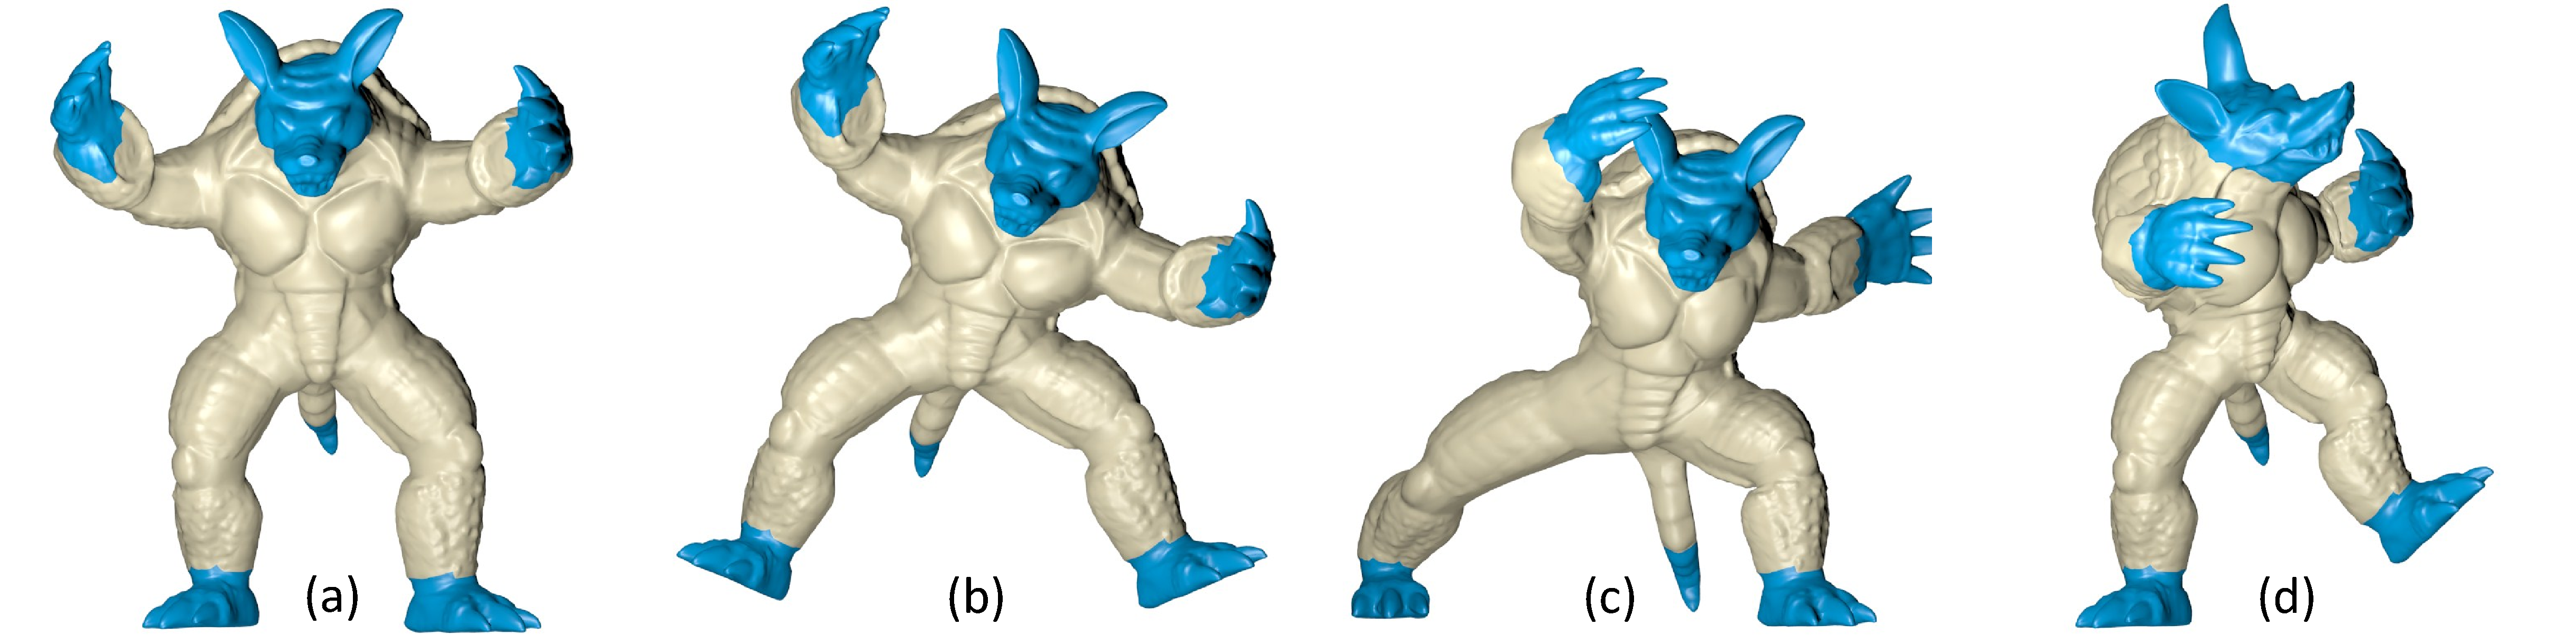
\includegraphics[width=1\textwidth]{img/Armadillo}
\par\end{centering}

\protect\caption{Anchor vertices in blue. (a) Original Model, (b,c,d) new poses only
change the anchor-vertices. The system finds positions for vertices
in yellow.}
\end{figure}


\end{frame}

\begin{frame}{3rd product - Results}


\framesubtitle{Mesh Editing with Laplacian Deform}


\begin{figure}[H]
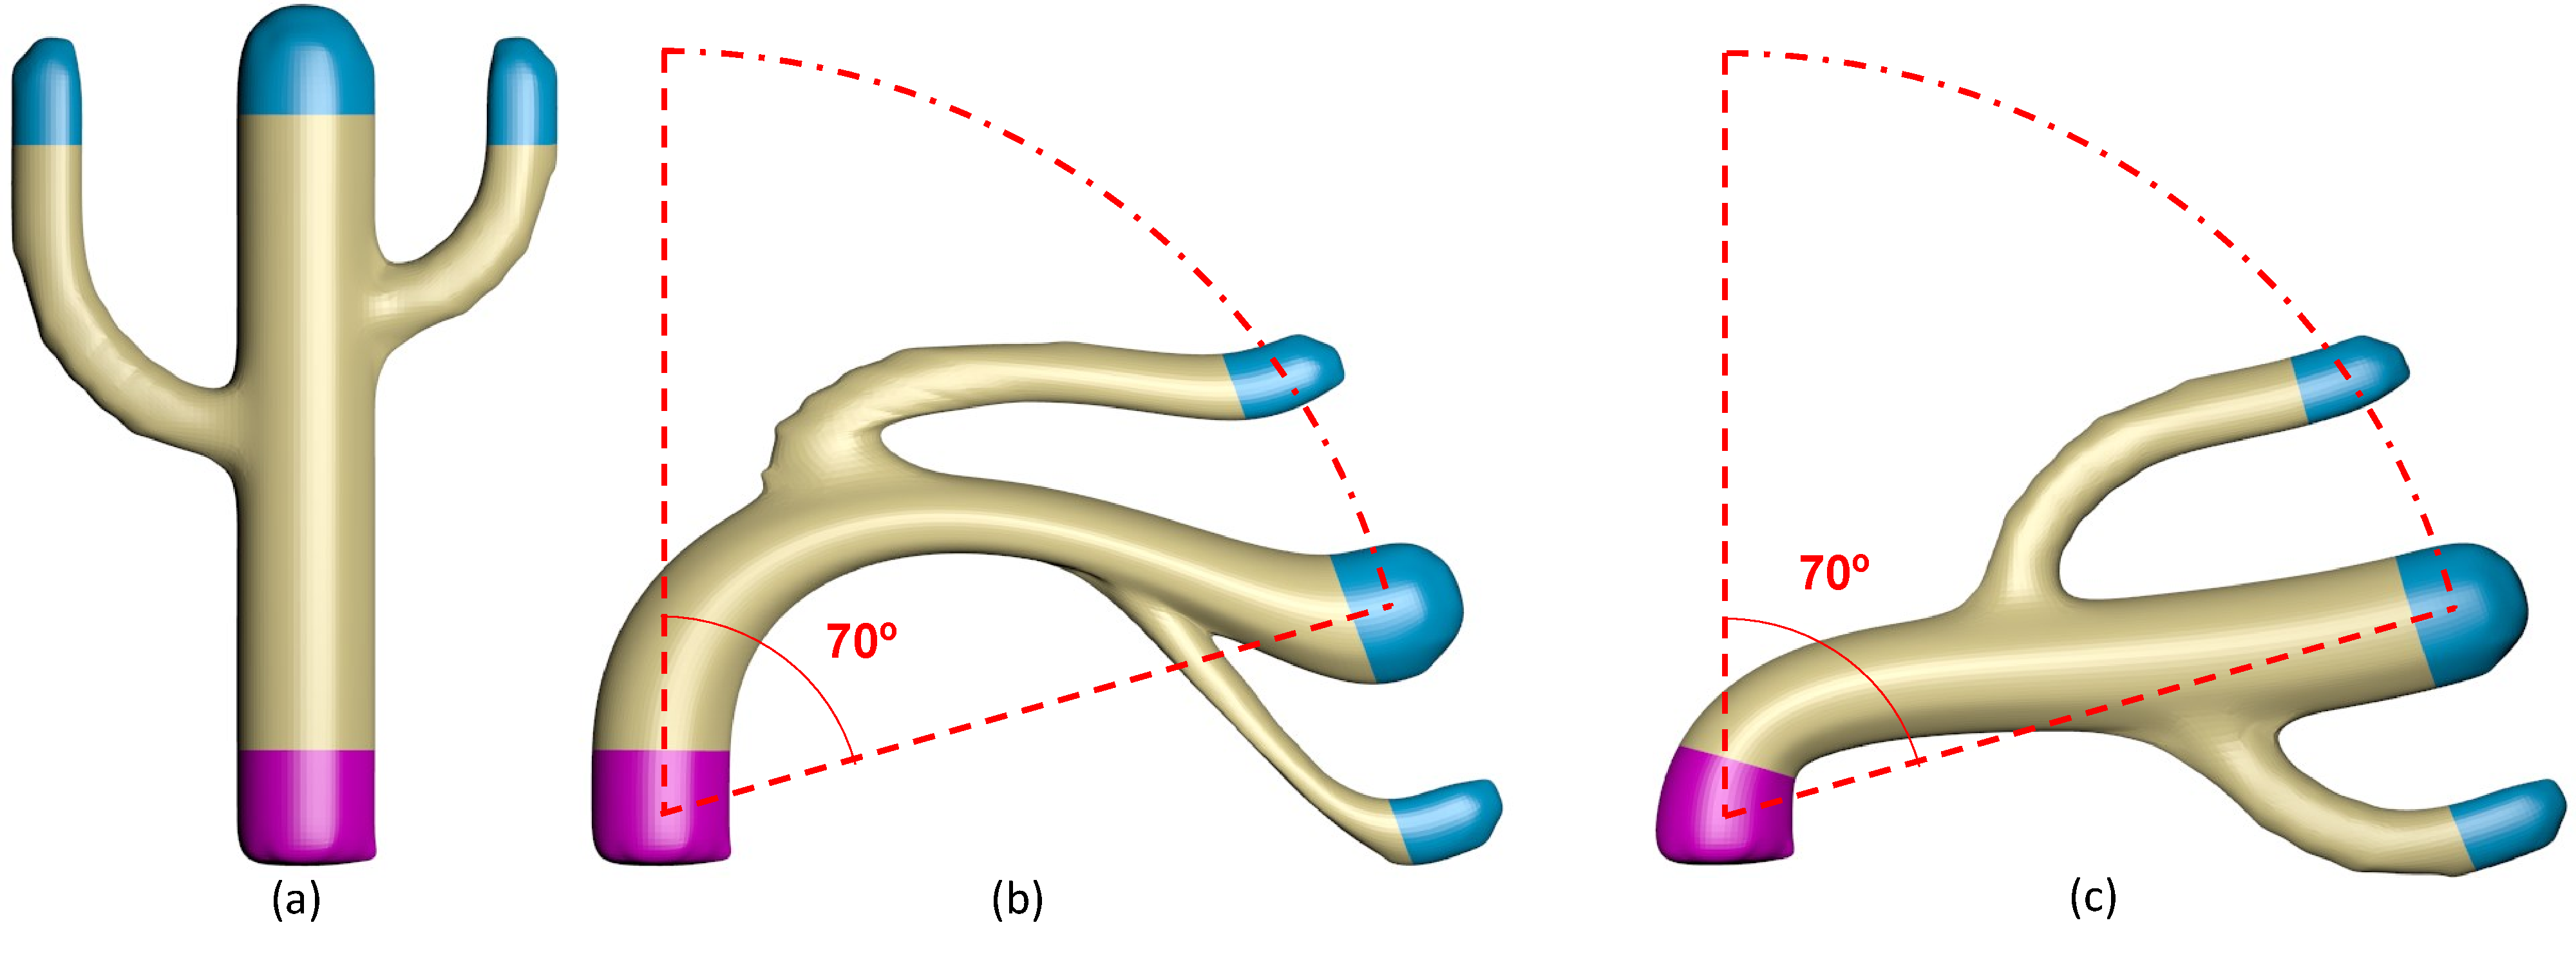
\includegraphics[width=1\textwidth]{img/cactus}

\protect\caption{(a) Original cactus model. (b) Blue segments are rotated 70º to the
right and, afterwards, a basic interpolation is applied to parts
in yellow (c) Blue segments are rotated 70º to the right and, afterwards,
a Laplacian deform tool is applied to parts in yellow.}
\end{figure}


\end{frame}

\begin{frame}{3rd product - Results}


\framesubtitle{Mesh Editing with Laplacian Deform}


\begin{figure}[H]
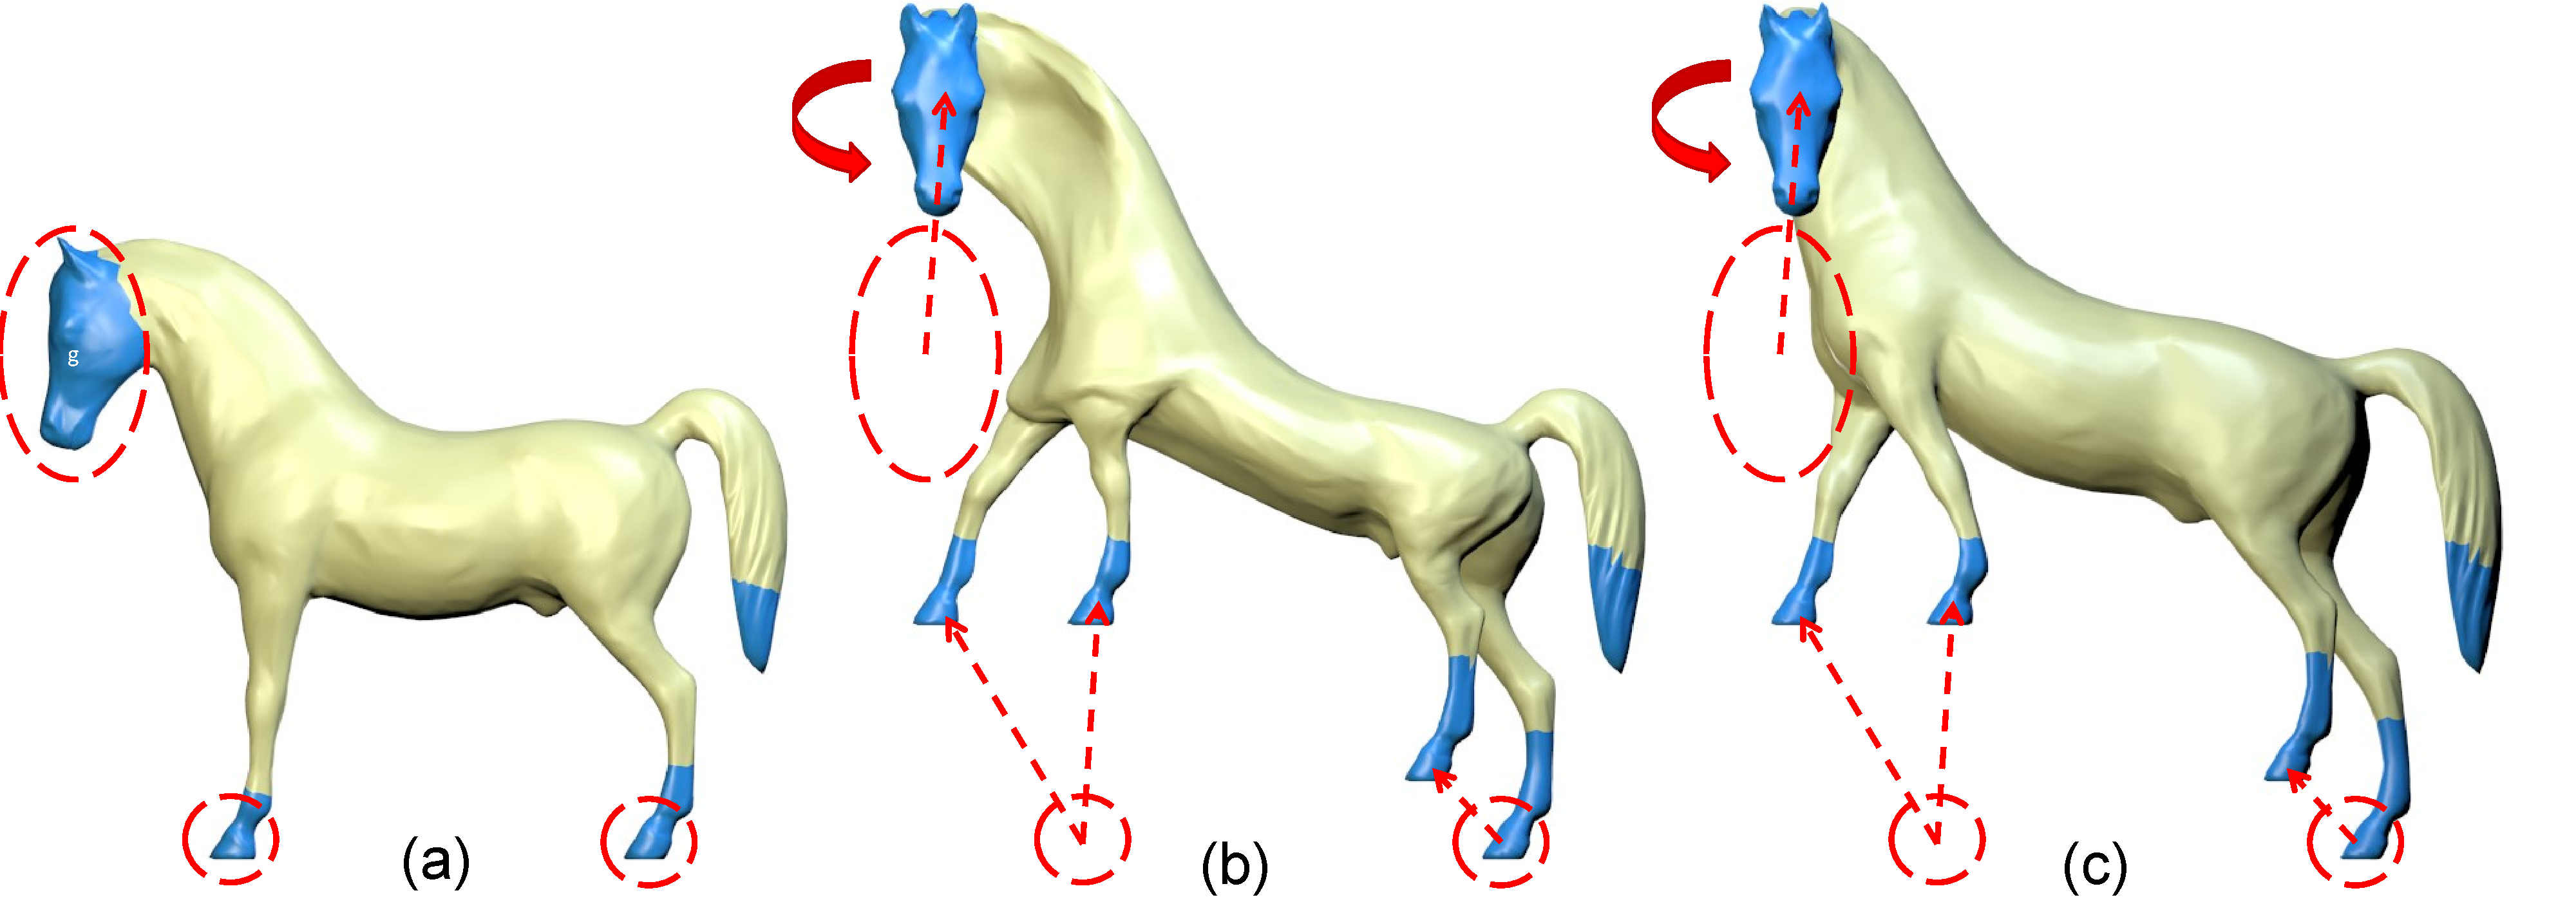
\includegraphics[width=1\textwidth]{img/horse}

\protect\caption{(a) Original Horse model. (b) Blue segments are translated and
rotated and then basic interpolation is applied to the yellow parts
(c) Blue segments are translated and rotated and then the Laplacian
Deform tool is applied to the yellow parts.}
\end{figure}


\end{frame} 



\begin{frame}{4th product - Poster}


\framesubtitle{{\small{}6th International Seminar on Medical Image Processing and
Analysis SIPAIM 2010}}


\noindent \begin{center}
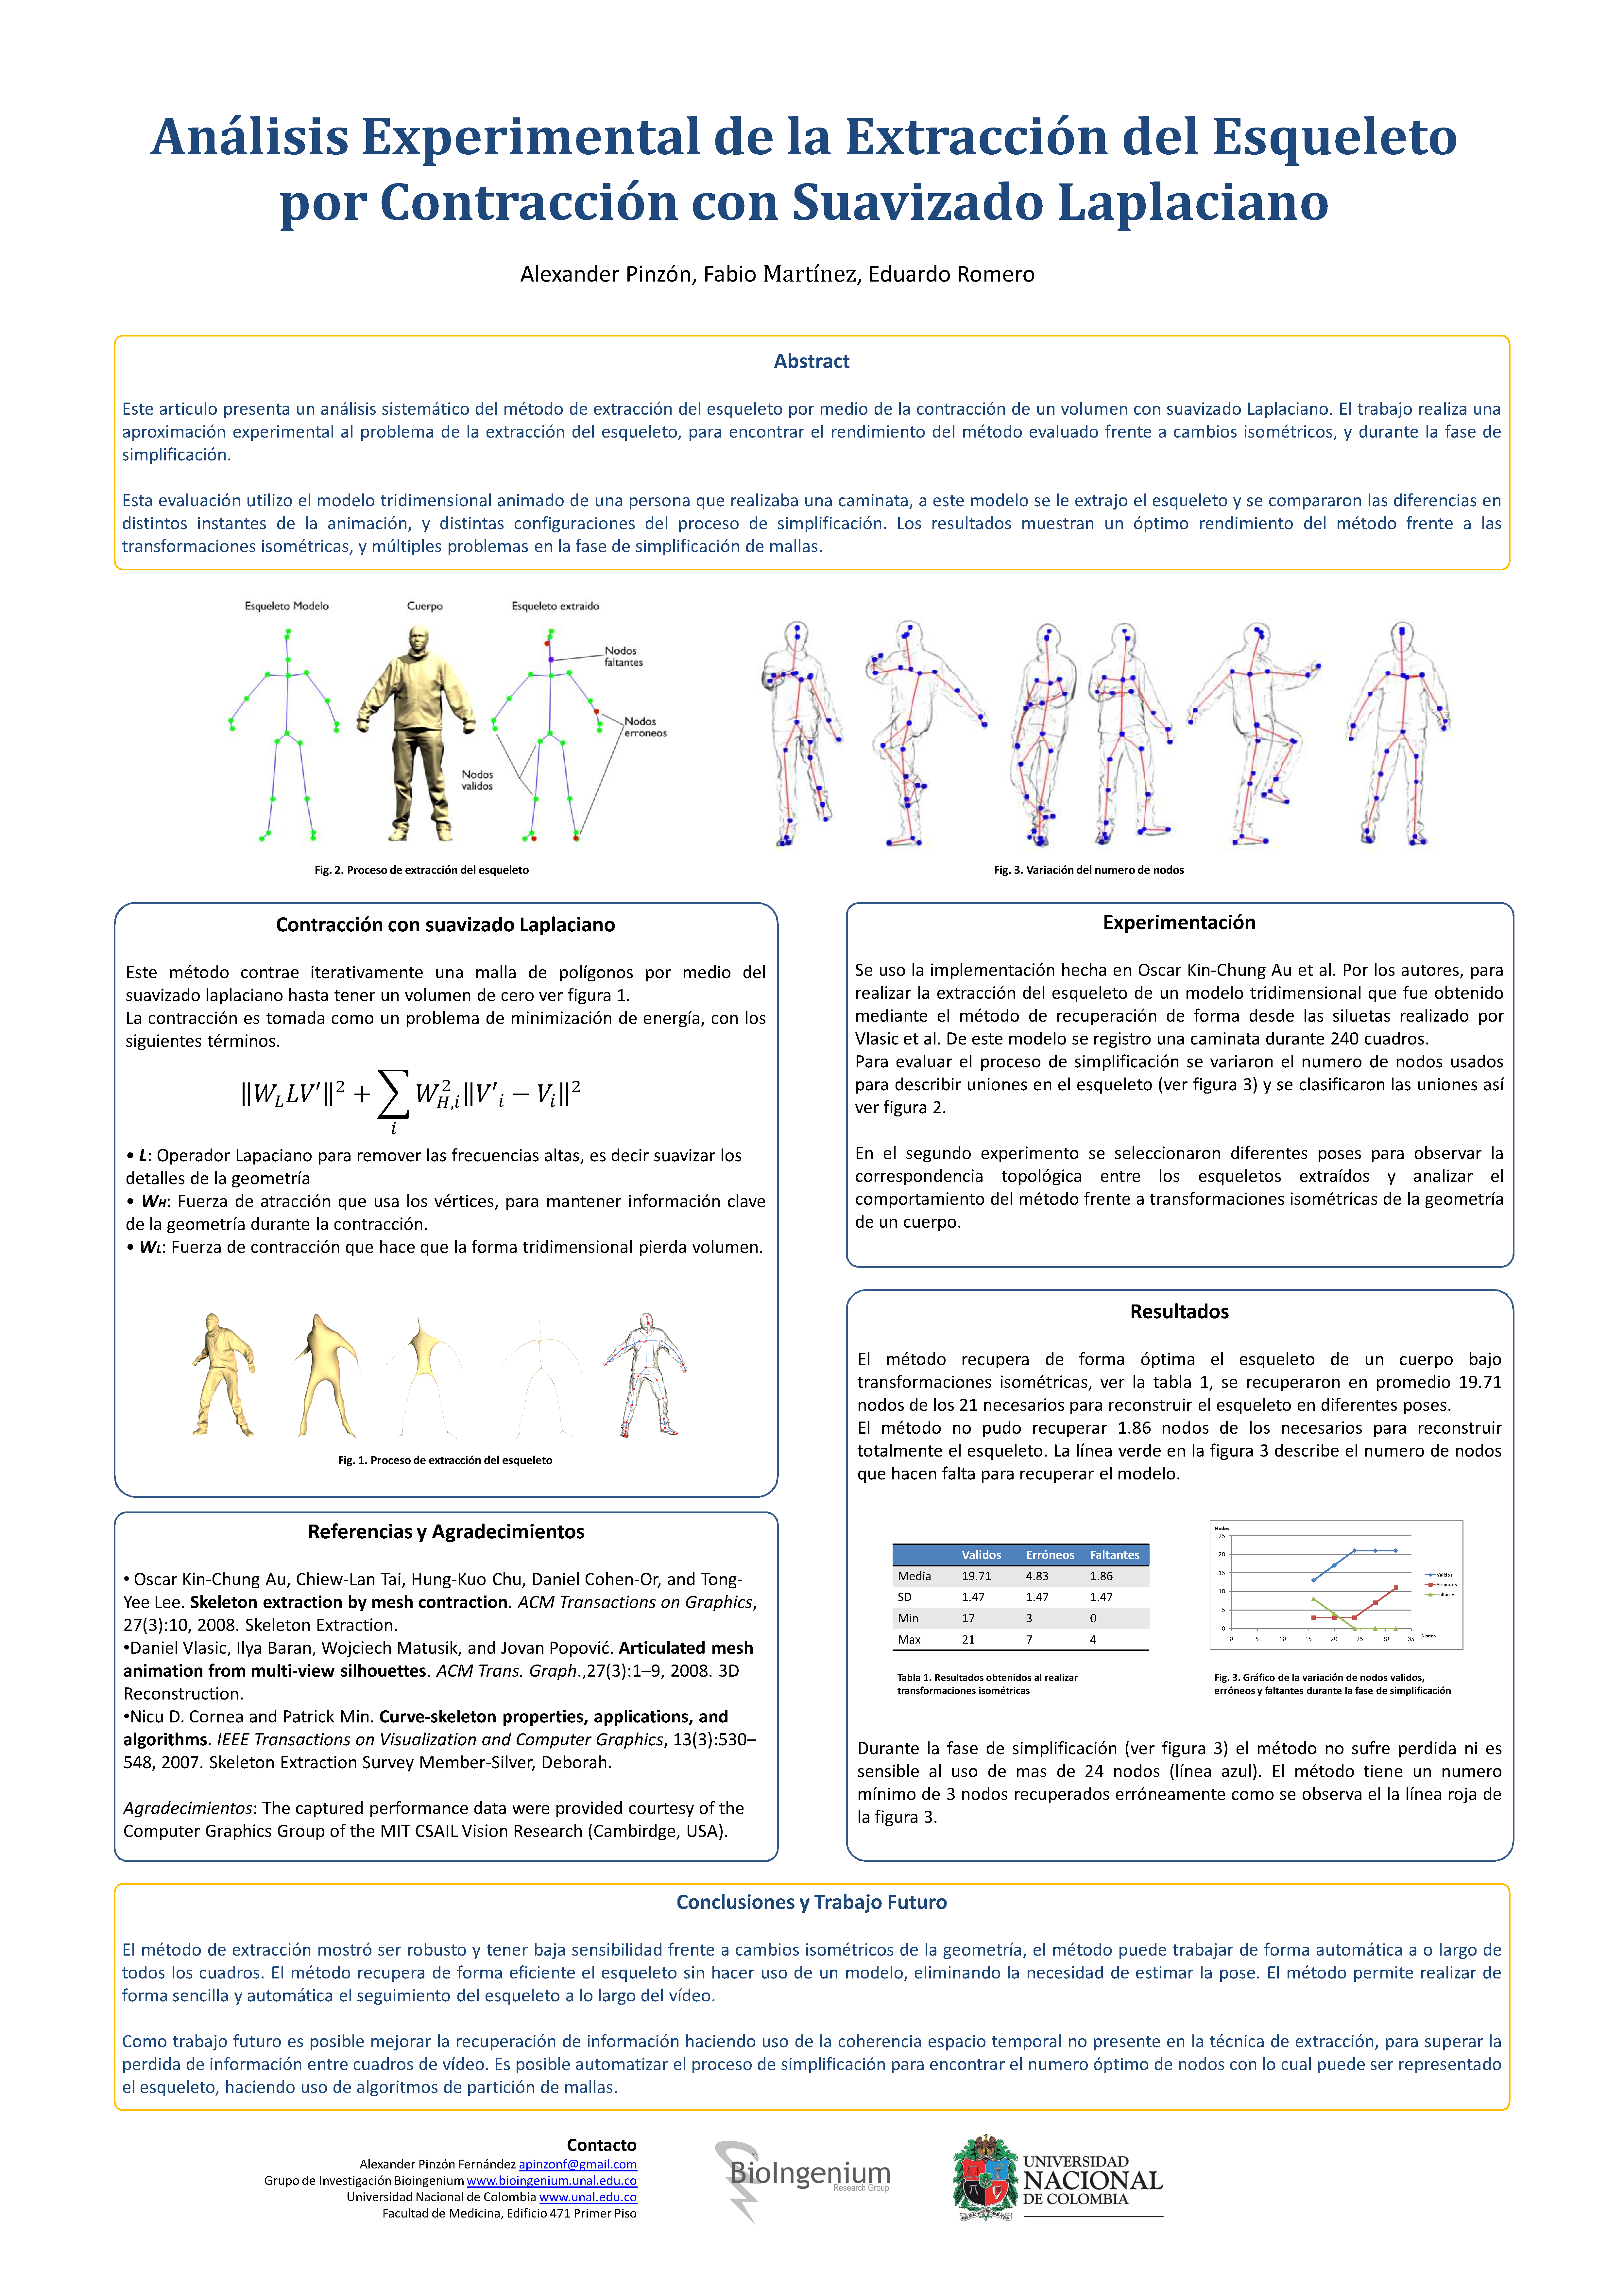
\includegraphics[height=0.8\textheight]{img/PosteraA0-150dpi}
\par\end{center}

\end{frame}

\begin{frame}{5th product - Poster}


\framesubtitle{{\small{}7th International Seminar on Medical Image Processing and
Analysis SIPAIM 2011}}


\noindent \begin{center}
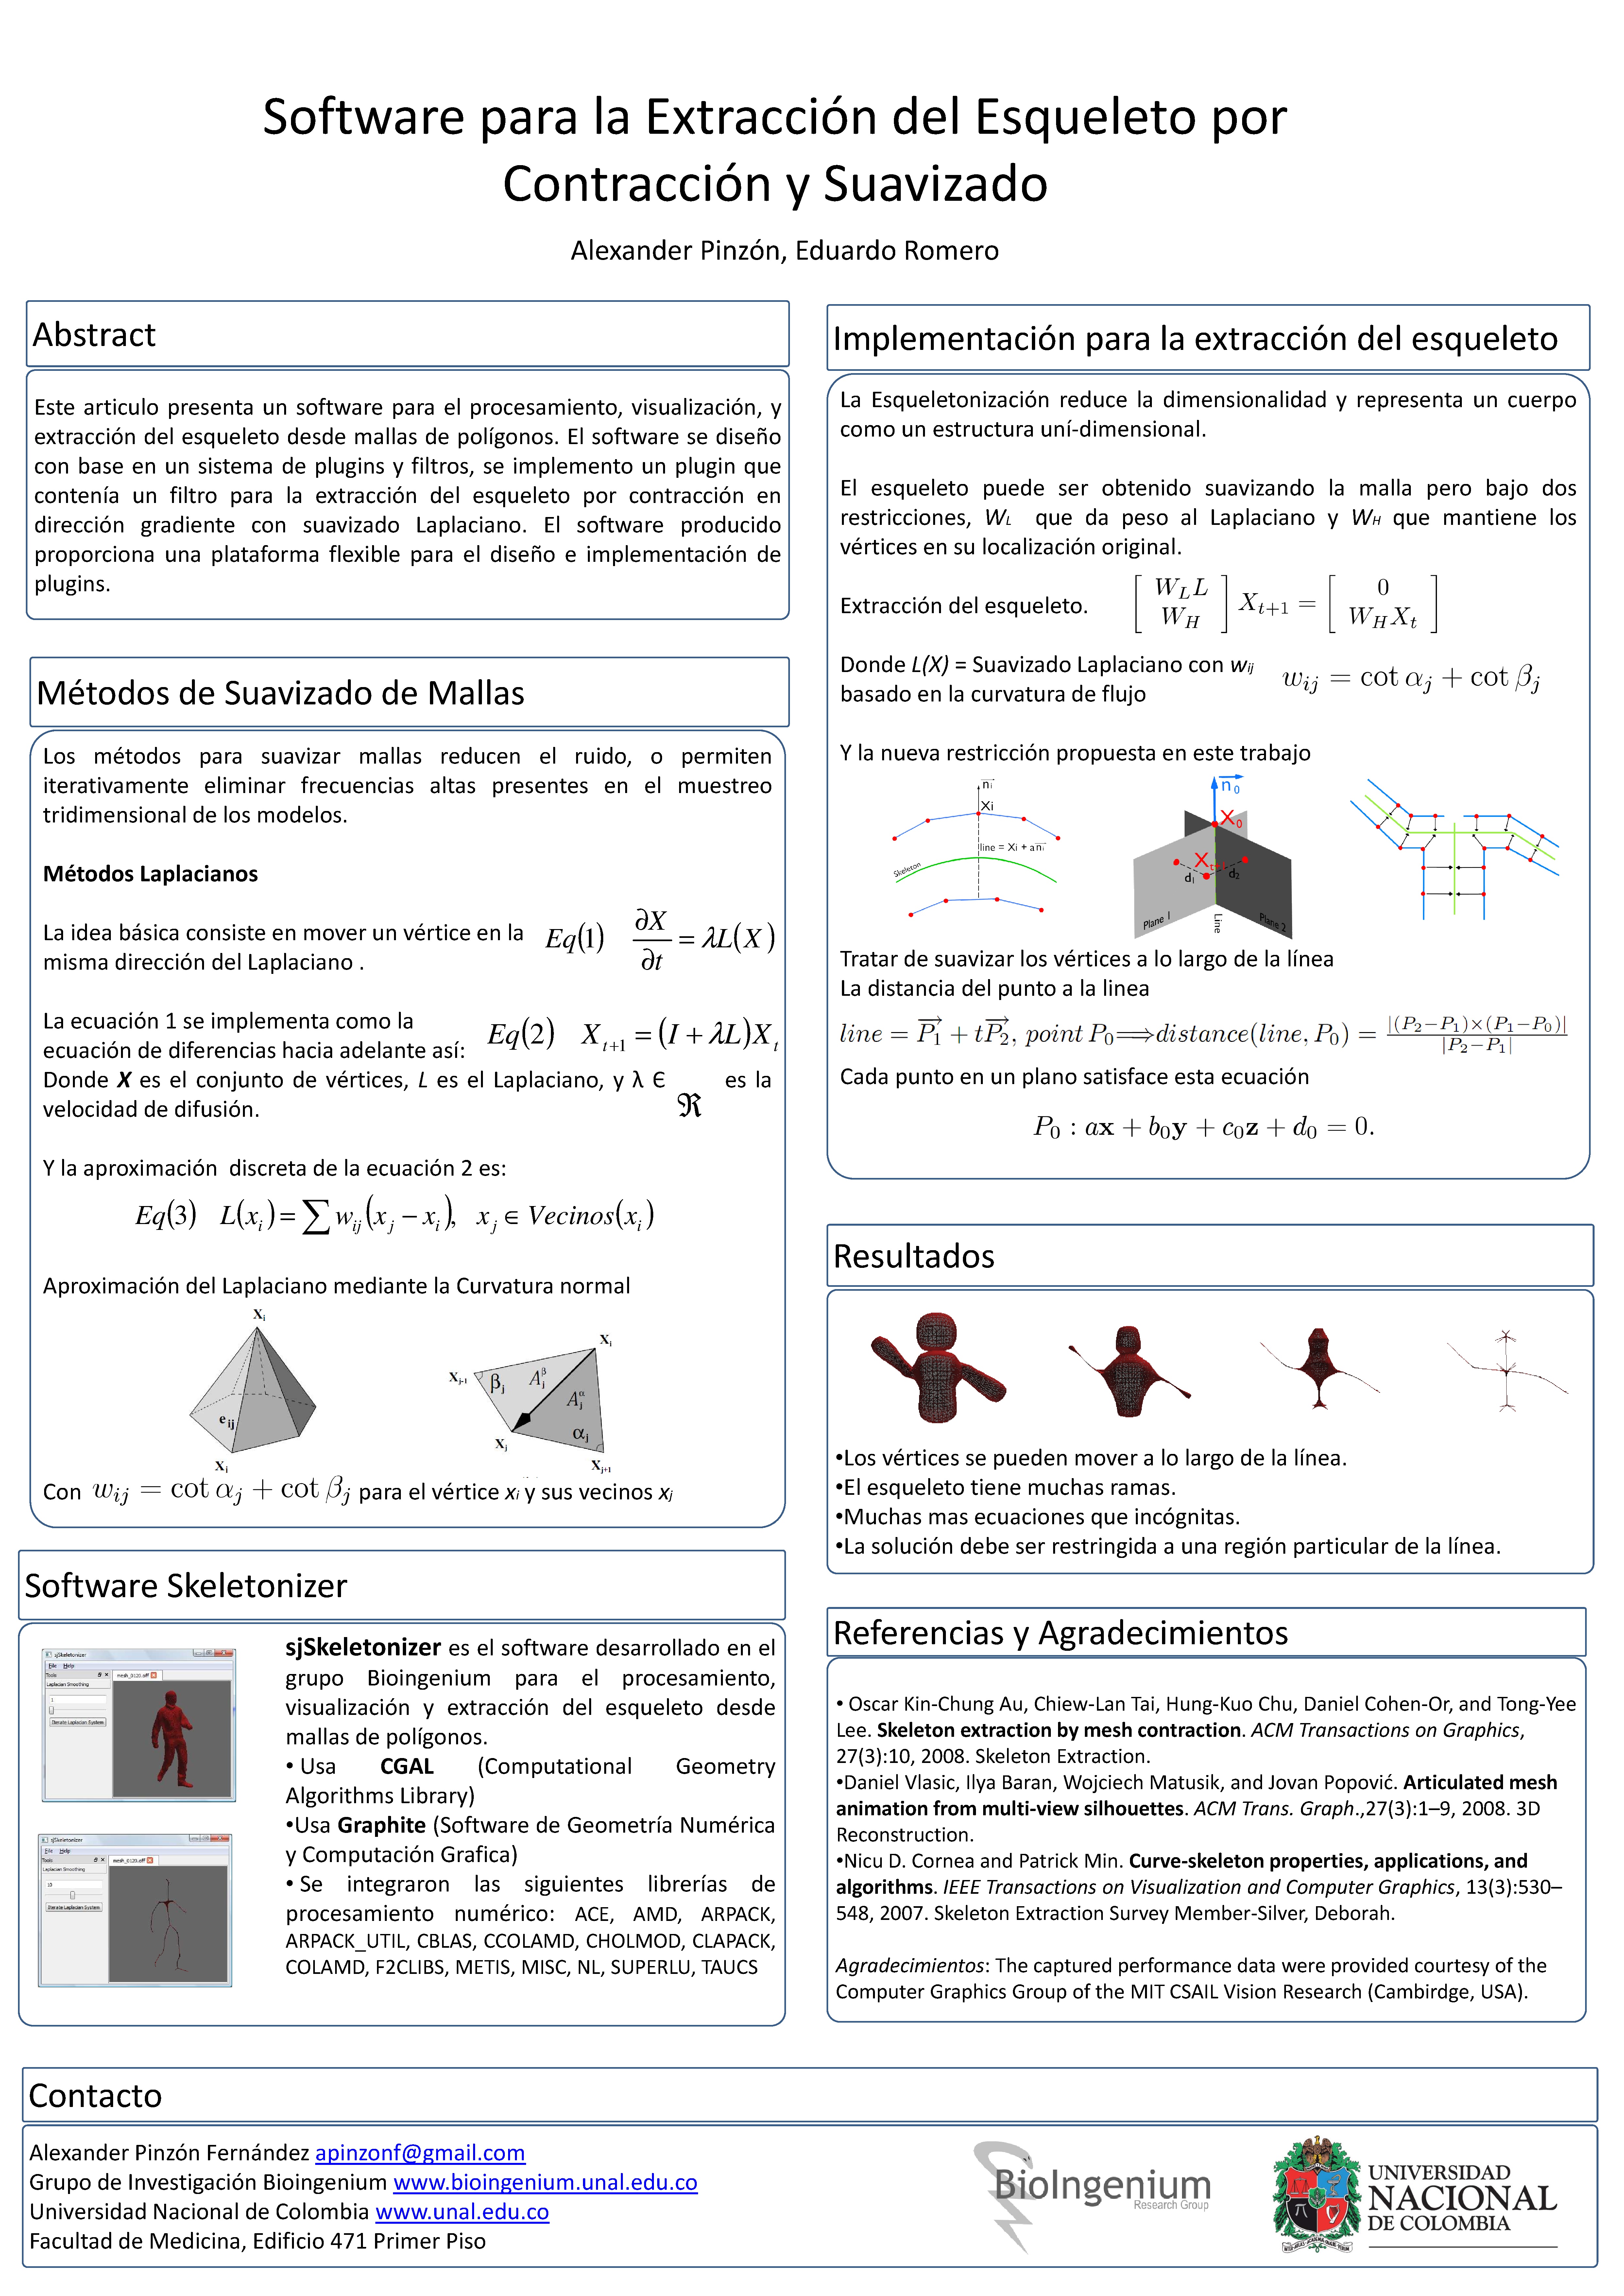
\includegraphics[height=0.8\textheight]{img/PosterSIPAIM2011}
\par\end{center}

\end{frame}

\begin{frame}{5th product - Skeleton extraction}


\framesubtitle{Software para la Extracción del Esqueleto por Contracción y Suavizado}


Au et al. {[}Au2008{]} propose the next system of equations to iteratively
contract the mesh until the volume is zero. Next, a simplification
process is done and a skeleton appears.


\begin{equation}
\left[\begin{array}{c}
W_{L}L\\
W_{H}
\end{array}\right]X_{t+1}=\left[\begin{array}{c}
0\\
W_{H}X_{t}
\end{array}\right]\label{eq:SkeletonExtraction}
\end{equation}

\begin{description}
\item [{$L$}] is a matrix that used our TQLBO defined in equation (\ref{eq:TQLBO_Laplacian_Matrix}). 
\item [{$W_{L}$}] is a diagonal weighting matrix for the smoothing factor.
\item [{$W_{H}$}] is a diagonal weighting matrix for the attraction constraint
factor. 
\item [{$A_{i}^{t}$~and~$A_{i}^{0}$}] are the current area and initial
area of the ring surrounding $x_{i}$.
\end{description}
\end{frame}



\begin{frame}{{\large{}Undesirable displacement of nodes from rotational center}}


%\framesubtitle{Software para la Extracción del Esqueleto por Contracción y Suavizado}
\framesubtitle{5th product - Poster}



\begin{figure}
\begin{centering}
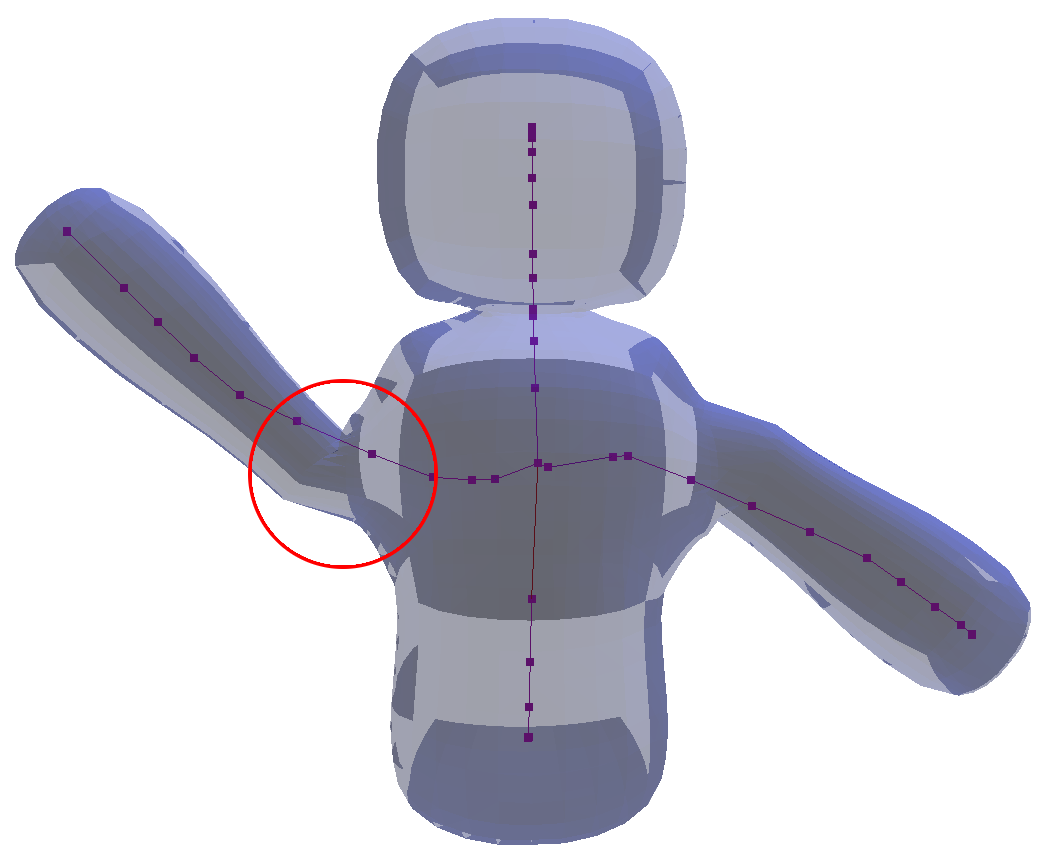
\includegraphics[width=0.5\textwidth]{img/skeleton_problem}
\par\end{centering}

\protect\caption{Skeleton that has a node outside its rotational center.}


\end{figure}


\end{frame}

\begin{frame}{5th product - Contribution}


\framesubtitle{Software para la Extracción del Esqueleto por Contracción y Suavizado}


The basic idea is to move the vertices along a normal line, estimated
at every vertex, based on the average of the normal of the faces. 


This constraint eliminates the need to adjust the final skeleton.


\begin{figure}[H]
\begin{centering}
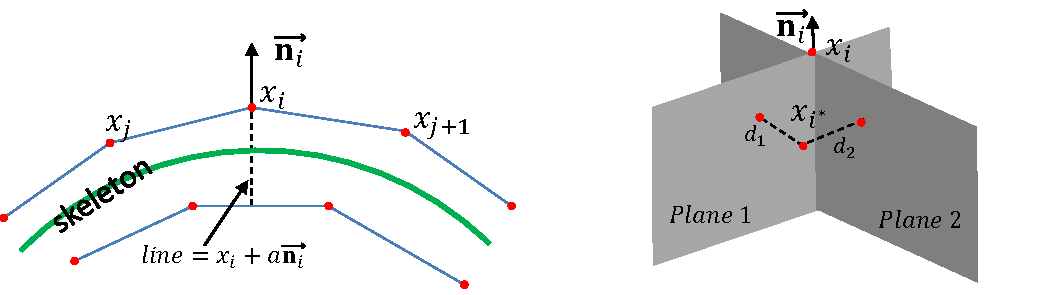
\includegraphics[width=1\textwidth]{img/LineConstraintSkeleton}
\par\end{centering}

\protect\caption{Left: The vertex $x_{i}$ moves along the line constraint. Right:
the distance of vertex $x_{i}$ to plane 1 and plane 2 when the position
in every iteration changes.}
\end{figure}


\end{frame}

\begin{frame}{The distance equation of point $p$ to plane $\Pi$}


%\framesubtitle{Software para la Extracción del Esqueleto por Contracción y Suavizado}
\framesubtitle{5th product - Poster}


The plane equation


\noindent \begin{center}
$a\mathbf{x}+b_{0}\mathbf{y}+c_{0}\mathbf{z}+d_{0}=0$
\par\end{center}


The distance of point $P_{0}=\{x_{0},y_{0},z_{0}\}$ to a plane $\Pi=a\mathbf{x}+b_{0}\mathbf{y}+c_{0}\mathbf{z}+d_{0}$.


\begin{equation}
\left|\Pi-P_{0}\right|=\frac{\left|ax_{0}+by_{0}+cz_{0}+d\right|}{\sqrt{a^{2}+b^{2}+c^{2}}}\label{eq:Plane_distance_equation}
\end{equation}



\note[item]{An equation plane only requires three non-collinear points$\left\{ P_{1},P_{2},P_{3}\right\} $
and we can solve the next system of equations to find the $a,b,c$
variables. usamos el vertice un desplazamietno alrededor de la normal
y otro vertice para calcular a b c.}

\end{frame}

\begin{frame}{5th product - The new system of equations proposed}


\framesubtitle{Software para la Extracción del Esqueleto por Contracción y Suavizado}
 

\begin{equation}
\left[\begin{array}{c}
W_{L}L\\
W_{H}\\
\Pi_{1}\\
\Pi_{2}
\end{array}\right]X_{t+1}=\left[\begin{array}{c}
0\\
W_{H}X_{t}\\
-D_{1}\\
-D_{2}
\end{array}\right]\label{eq:SkeletonExtractionDistance}
\end{equation}

\begin{description}
\item [{$\Pi_{1}$~and~$\Pi_{2}$}] are matrices that contain $a,b,c$
values of the plane equation for every vertex. 
\item [{$D_{1}$~and~$D_{2}$}] are the vectors with $d$ values of the
plane equation for every vertex.
\end{description}
\end{frame}




\begin{frame}{5th product - User interface}


\framesubtitle{Software para la Extracción del Esqueleto por Contracción y Suavizado}


\begin{figure}
\begin{centering}
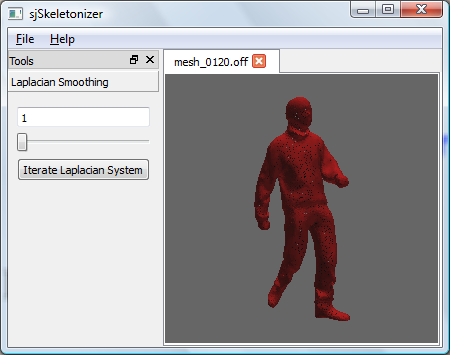
\includegraphics[width=0.4\textwidth]{img/sjSkeletonizer01}~~~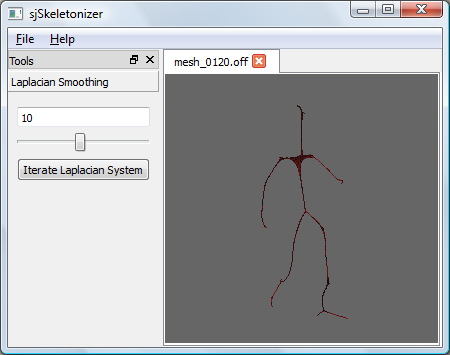
\includegraphics[width=0.4\textwidth]{img/sjSkeletonizer02}
\par\end{centering}

\protect\caption{sjSkeletonizer is our prototype software application}


\end{figure}



As a result of this work, the software sjSkeletonizer permits the
processing, visualization and extraction of the skeleton from polygonal
hybrid meshes composed of triangles and quads.

\end{frame}

\begin{frame}{5th product - Results}


\framesubtitle{Software para la Extracción del Esqueleto por Contracción y Suavizado}


\begin{figure}[H]
\begin{centering}
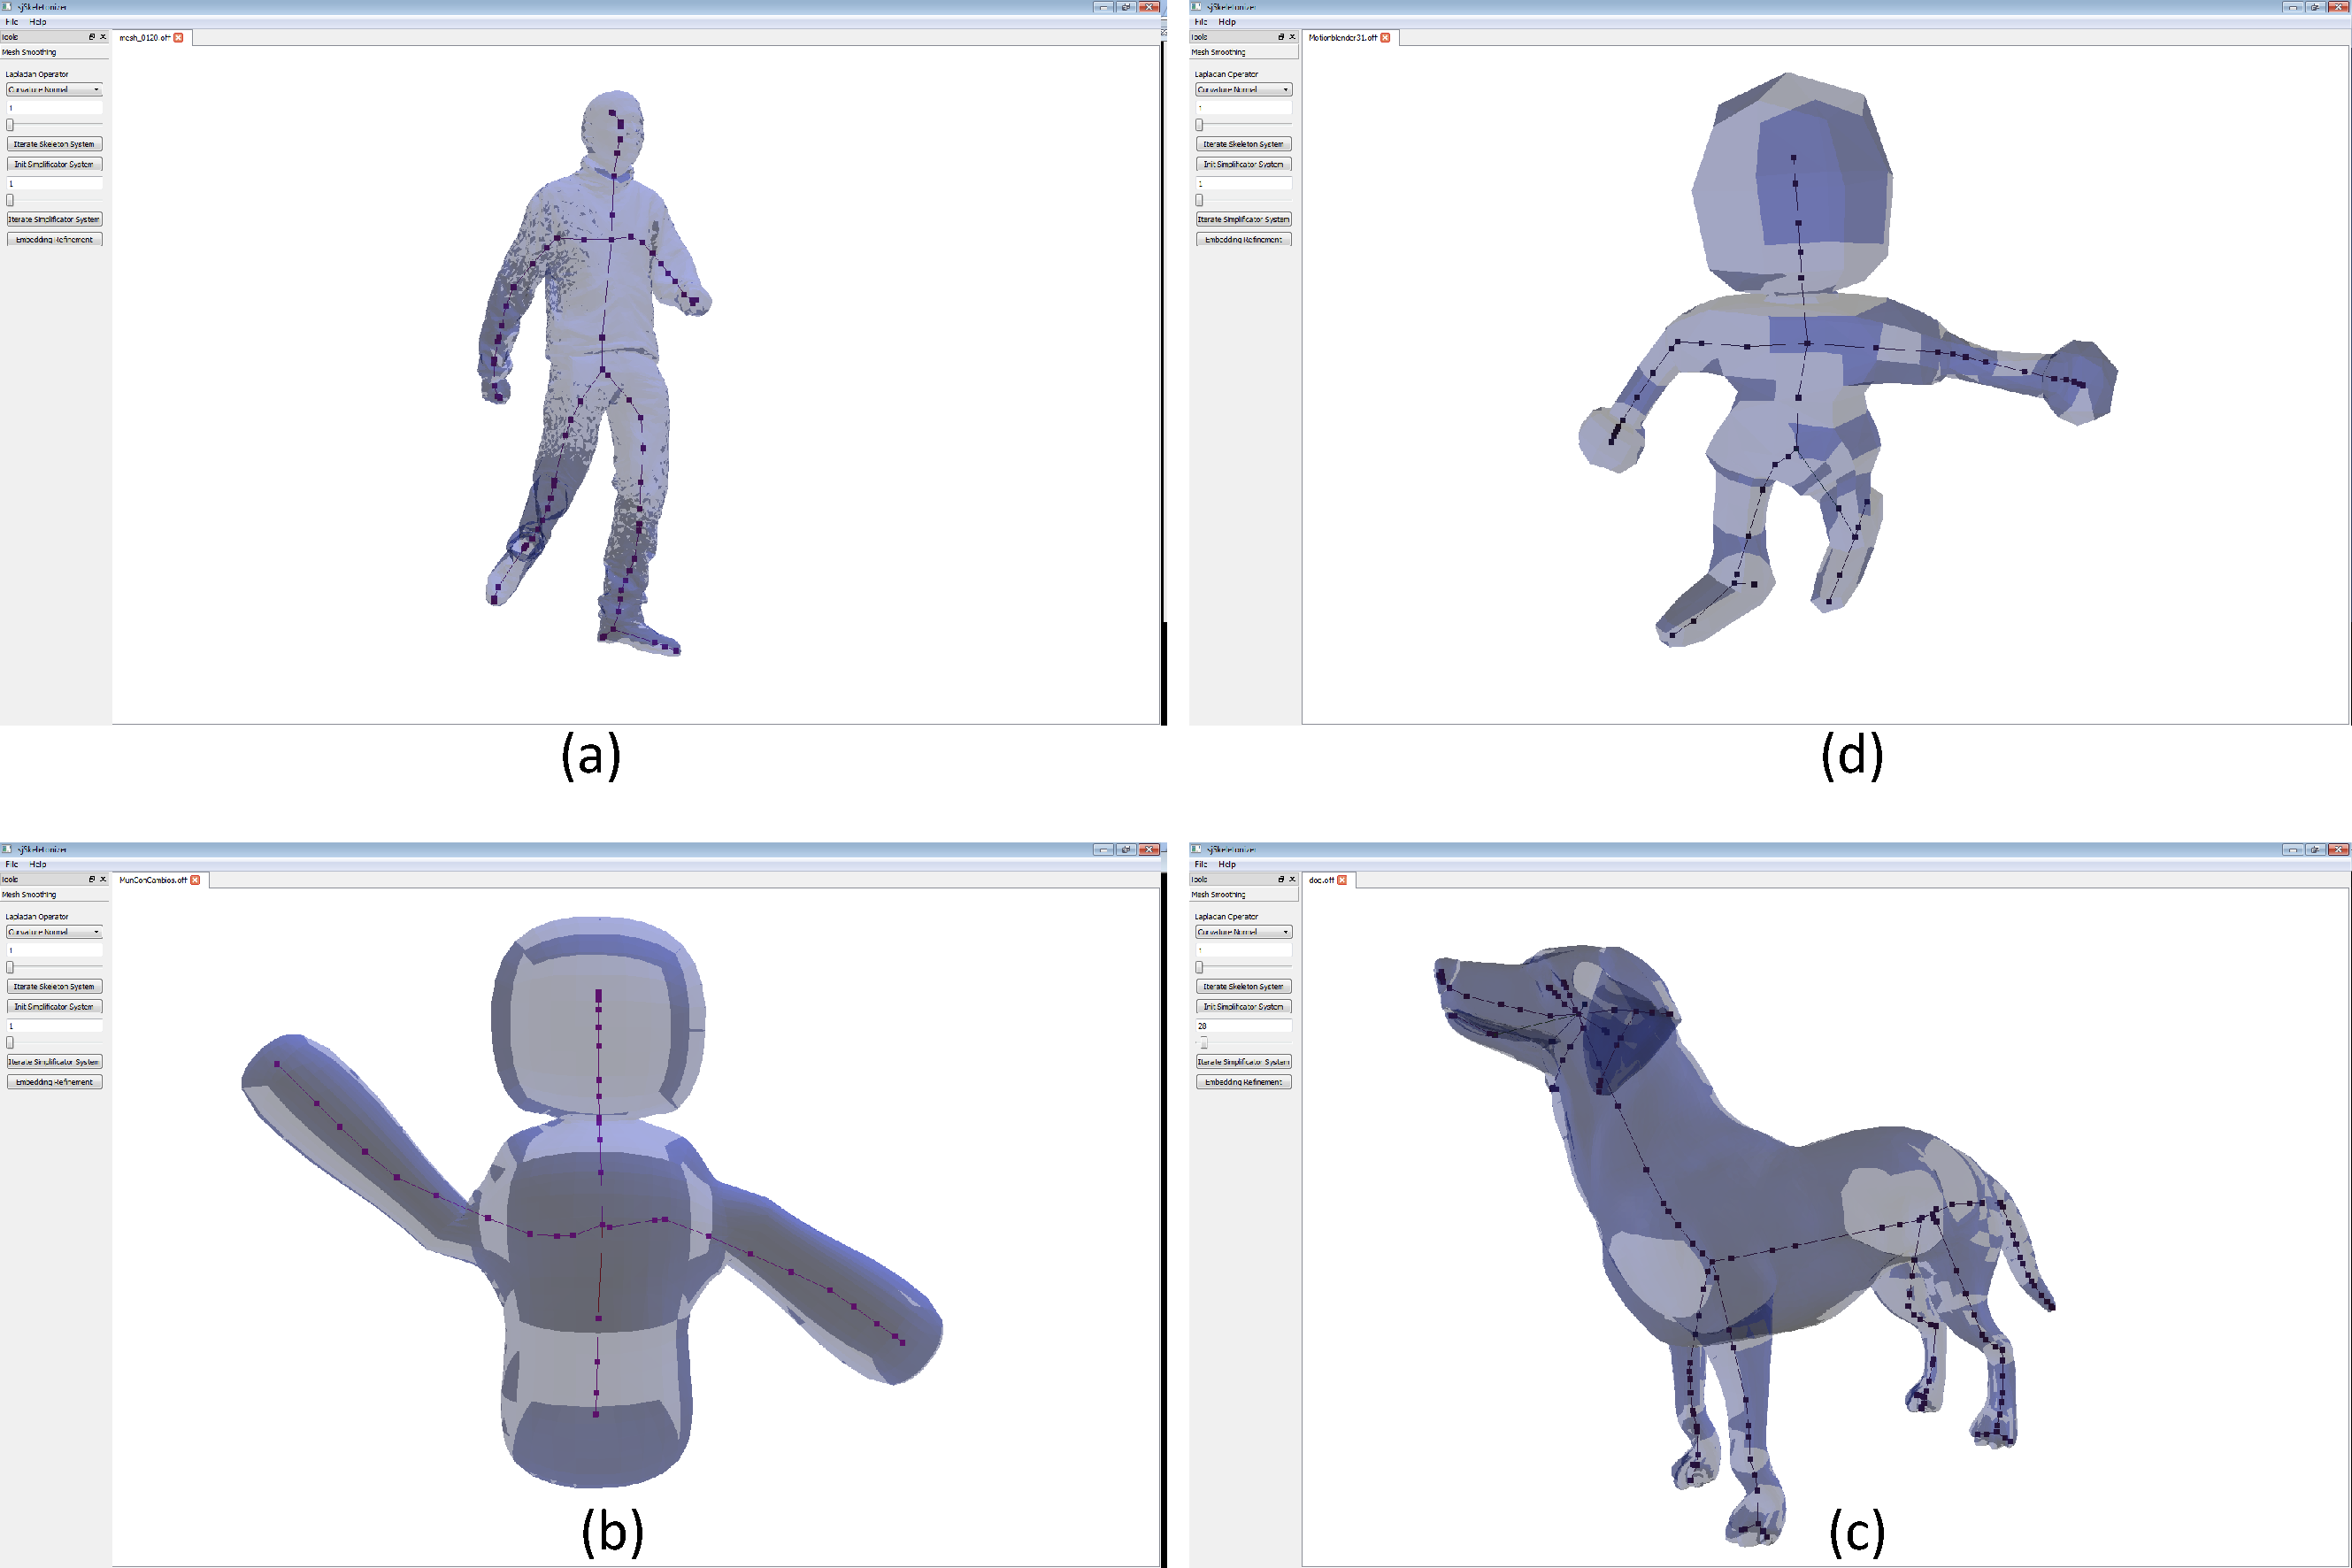
\includegraphics[width=0.7\textwidth]{img/Skeletonizer_2}
\par\end{centering}

\protect\caption{Skeletons extracted from different models. (a) Dog model (b) Character
model. (c) Person model. (d) Clay model.}
\end{figure}


\end{frame}
 

\begin{frame}{5th product - Results}


\framesubtitle{Software para la Extracción del Esqueleto por Contracción y Suavizado}


\begin{figure}[H]
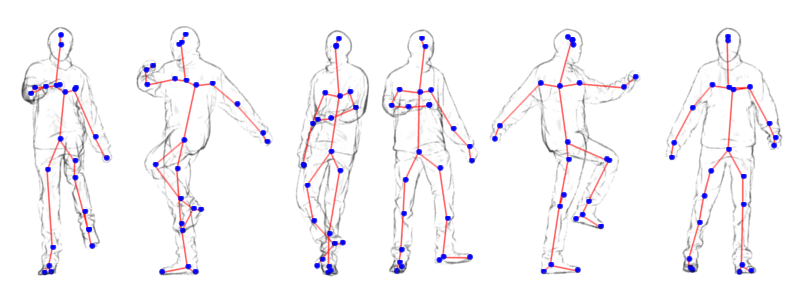
\includegraphics[width=0.8\textwidth]{img/poses}

\protect\caption{Model with different poses and skeleton obtained with our skeleton
extraction software.}
\end{figure}


\end{frame}


\section{Conclusions}
\begin{frame}{Conclusions}

\begin{itemize}
\item This work presented a novel extension of the Laplace Beltrami operator
for hybrid quad/triangle meshes, and the successful application of
such principles in different types of problems in computer geometric
modeling like smoothing, enhancing, sculpting, deformation, reposing
and skeleton extraction.
\pause{}
\item A new sculpting brush to made a proper inflation while preserving
the geometric details in real-time sessions was proposed, implemented
and tested.
\pause{}
\item We have largely demonstrated that our method has a good performance,
stability and robustness of the extension proposed.
\pause{}
\item This novel extension of the Laplace Beltrami operator was introduced
in the computer modeling industry inside the Blender 3D computer graphics
software.
\end{itemize}
\end{frame}

\begin{frame}{Acknowledgment}

\begin{itemize}
\item We would like to thank CIM@LAB Research Group for their support on
our research.
\item This work was supported in part by the Blender Foundation, Google
Summer of code program in 2012 and 2013. 
\item Livingstone elephant model was provided by courtesy of INRIA and ISTI
by the AIM@SHAPE Shape Repository. Hand model was courtesy of the FarField
Technology Ltd. Camel model by Valera Ivanov is licensed under a Creative
Commons Attribution 3.0 Unported License. Dinosaur and Monkey models
are under public domain, courtesy of Blender Foundation.
\end{itemize}

\end{frame}

 \begin{frame}[allowframebreaks]{Bibliography}


{\scriptsize{}\bibliographystyle{plain}
\nocite{*}
\bibliography{bibliography}
}{\scriptsize \par}

\end{frame}
 

\plain{
Thank you for coming today\\
\vspace{5pt}
Questions?}
 
\end{document}